\documentclass{article}
\usepackage{amsthm}
\usepackage{amsmath}
\usepackage{graphicx}
\usepackage{color}
\usepackage{subfig}
\usepackage{physics}
\graphicspath{ {figures/} }

\title{Monte Carlo Methods}
\author{Caitlin Carnahan}
\begin{document}
This document is intended to serve as personal notes
for self-study of \emph{Monte Carlo Methods for Statistical Physics}
by M.E.J. Newman and G.T. Barkema.

\section{Introduction}
\subsection{Statistical Mechanics}
Many systems of interest are composed of very many simple
constituent systems. For example, a liter of oxygen
is composed of $~10^{22}$ oxygen molecules. The equations
of motion for a single oxygen molecule are relatively simple
but the sheer number of oxygen molecules in the larger system
render the exact solutions infeasible. Instead, we approach
the larger system via probabilistic methods. The goal is to
express the state of the larger system as a set of probabilities
of being in one state or another.

The typical systems studied in physics for which MCM are useful
are systems described by a Hamiltonian $H$ and an
associated energy spectrum that is either continuous or given
by a discrete set $E_{0}$, $E_{1}$, $E_{2}$, etc. We will also
consider systems that interact with a thermal reservoir with
which the system can exchange heat. Heat exchanges with the
reservoir manifest as a small (negligible) perturbation
in the Hamiltonian which pushes the system from one energy
state to another.

Modeling the effect of the perturbation on the Hamiltonian is
done by defining a \emph{dynamics} for the system. The dynamics
of the system may take the form of a set of transition rates.
Suppose the system is in a state $\mu$. Then, $R(\mu \rightarrow \nu)dt$ is
defined to be the probability that the system transitions to a state
$\nu$ in time $dt$, where $R(\mu \rightarrow \nu)$ is defined to be the
\emph{transition rate}. We may also define a set of weights $w_{\mu}(t)$
which represent that probability that the system will be found in state
$\mu$ at time $t$. Using these elements, we can write down a \emph{master
equation}:
\begin{equation}
\frac{dw_{\mu}}{dt} = \sum_{\nu}[w_{\nu}(t)R(\nu \rightarrow \mu)
                              - w_{\mu}(t)R(\mu \rightarrow \nu)]
\end{equation}
The first term in the sum is the rate at which the system is
transitioning into state $\mu$. The second term is the rate at which
the system is transitioning out of state $\mu$.

We may define the expectation value of some observable $Q$, which
takes the value $Q_{\mu}$ in state $\mu$, as
$$ \left \langle Q \right \rangle = \sum_{\mu} Q_{\mu}w_{\mu}(t) $$
The expectation value of $Q$ can be interpreted two ways:
\begin{itemize}
\item It is the mean of the observed value of $Q$ that would be
obtained if we measured many identically prepared systems simultaneously.
\item It is the time average of the quantity $Q$. That is, it might be the
average observed value of $Q$ after many measurements over time.
\end{itemize}

\subsection{Equilibrium}
An \emph{equilibrium} state can be defined as a state in which all of the
rates of change $dw_{\mu}/dt$ vanish, and therefore the transition rate
into and out of each state $\mu$ must be equal. All systems goverened
by the master equation must come to equilibrium after some time and so
we can define the equilibrium values of the weights, the
\emph{equilibrium occupation probabilities}, as
$$p_{\mu} = \lim_{t\rightarrow \infty} w_{\mu}(t)$$
For a system in equilibrium with thermal reservoir at temperature T, the
Boltzmann distribution is
$$p_{\mu} = \frac{1}{Z}e^{-E_{\mu}/kT} = \frac{1}{Z}e^{-\beta E_{\mu}}$$
where $Z$ is the normalization constant, called the \emph{partition function}, and
defined as
$$Z = \sum_{\mu}e^{-\beta E_{\mu}}$$
Plugging this into our definition of expectation values gives us
$$ \left \langle Q \right \rangle = \sum_{\mu} Q_{\mu}p_{\mu}(t)
                                  = \frac{1}{Z}\sum_{\mu} Q_{\mu}e^{-\beta E_{\mu}} $$
which is the expression for the expectation value of a system in equilibrium.
For example, the internal energy $U$ of a system is given by
$$U = \left \langle E \right \rangle
                                  = \frac{1}{Z}\sum_{\mu} E_{\mu}e^{-\beta E_{\mu}}
                                  = -\frac{1}{Z}\frac{\partial Z}{\partial \beta}
                                  = -\frac{\partial log Z}{\partial \beta}$$
It is sometimes appropriate in MCM calculations to calculate the partition function, from which
many other quantities can be derived. Some examples can be found in Section 1.2 of Newman and
Barkema.

\subsection{Fluctuations, Correlations, and Responses}
It is useful to assess the fluctuations in observable quantities. Doing so
allows us to determine how the quantity we are measuring varies over time and
therefore how much of an approximation is being made by calculating the expectation
value. As an example, the root-mean-square fluctuation in internal energy is given by
$$\sqrt{\left \langle E^{2} \right \rangle - \left \langle E \right \rangle^{2}} = \sqrt{\frac{\partial^{2}log Z}{\partial \beta^{2}}}$$
In the limit of a large system, called the \emph{thermodynamic limit}, it is common for
fluctuations to become negligible. For example, RMS fluctuations in internal energy scale
as $\sqrt{V}$ in a system of volume $V$, but the internal energy itself scales as $V$
so as the system becomes very large, the fluctuations grow increasingly
negligible.

Every parameter that can be fixed in a system (e.g. volume, external field)
has a conjugate variable (e.g. pressure, magnetization) that is given by a
derivative of the free energy. For example,
$$ p = -\frac{\partial F}{\partial V}$$
$$ M = \frac{\partial F}{\partial B}$$
The Hamiltonian contains terms of the form $-XY$ where $Y$ is a "field" whose
value is fixed, and $X$ is the conjugate variable to which it couples.
A common trick to calculate the thermal average of a quantity is the following:
\begin{itemize}
\item Make up a fictitious field that couples to the quantity of interest.
\item Add an appropriate term to the Hamiltonian.
\item Set the field to zero after performing the derivative on the free energy.
\end{itemize}
The \emph{susceptibility} of $X$ to $Y$ is a measurement of the strength of
the response of $X$ to variation in $Y$. Typically, this quantity is denoted
by $\chi$ and can be defined as
$$\chi = \frac{\partial \left \langle X \right \rangle  }{\partial Y}$$
The \emph{linear response theorem} tell us that the fluctuations in a variable
are proportional to the susceptibility of the variable to its conjugate field.

\subsubsection{Correlation Functions}
The \emph{disconnected correlation function} $G^{(2)}(i,j)$ is defined as
$$G^{(2)}(i,j) = \left \langle x_{i}x_{j} \right \rangle$$
This function gives us roughly an idea of how the variables $x_{i}$ and $x_{j}$
are correlated. Consider the following scenarios:
\begin{itemize}
\item If $x_{i}$ and $x_{j}$ move (roughly) together most of the time around
the origin zero, then the average of their product will be a positive value.
\item If $x_{i}$ and $x_{j}$ move (roughly) together but in opposite dirrections
most of the time, then the average of their product will be a negative value.
\item If $x_{i}$ and $x_{j}$ move with no discernible pattern relative to one
another, then their product will be sometimes positive and sometimes negative,
averaging to zero over a long time.
\end{itemize}

This definition can be problematic in the case of a \emph{spontaneously
broken symmetry state}. This occurs when a variable $x$ develops a non-zero
expectation value. If this happens, $x_{i}$ and $x_{j}$ may, for instance,
always be large positive values leading to a large positive correlation value
even if they have nothing to do with one another. To address this problem, we
can use the \emph{two-point connected correlation function} $G_{c}^{(2)}(i,j)$
defined as
$$G_{c}^{(2)}(i,j) = \left \langle x_{i}x_{j} \right \rangle - \left \langle x_{i} \right \rangle \left \langle x_{j} \right \rangle$$
$$ = \left \langle (x_{i} - \left \langle x_{i} \right \rangle) \times (x_{j} - \left \langle x_{j} \right \rangle) \right \rangle $$
For reference, the higher-order connected correlation functions for three and four sites can be found in
section 1.2.1.

\subsection{Example: The Ising Model}
The two-dimensional Ising model of a magnet consists of a lattice of sites, where
each site contains a magnetic dipole or spin. Each spin is a two-level system
denoted by the variable $s_{i}$, which can only take on the values $\pm 1$. Exchange
interactions are modeled by including terms proportional to $s_{i}s_{j}$ in the
Hamiltonian. In the simplest case, these terms are identical for each pair of spins
(indicating the same interaction strength $J$ all over the lattice). Another simplification
is to consider only nearest neighbor interactions. An external magnetic field $B$
can also be introduced. In this case we obtain the following Hamiltonian
$$H = -J\sum_{\left \langle ij \right \rangle }s_{i}s_{j} - B\sum_{i}s_{i}$$
where $\left \langle ij \right \rangle$ indicates a sum over nearest neighbors. The minus
signs are conventional and fix the signs of the parameters $J$ and $B$. In the current form:
\begin{itemize}
\item A positive $J$ value (\emph{ferromagnetic}) makes the spins want to align to minimize the Hamiltonian.
\item A negative $J$ value (\emph{anti-ferromagnetic}) makes the spins want to anti-align.
\item A positive $B$ value makes the spins want to orient positively.
\item A negative $B$ value makes the spins want to orient negatively - that is, they
want to align with the magnetic field.
\end{itemize}
Each state of the Ising system is an specific "setting" of the spins in the lattice. For $N$
sites in the lattice, there are $2^{N}$ states. Earlier we defined the partition function
$Z$ as
$$Z = \sum_{\mu}e^{-\beta E_{\mu}}$$
where \{$\mu$\} represents a set of states. So our Ising partition function is given by
$$Z = \sum_{s_{1} = \pm 1} \sum_{s_{2} = \pm 1}...\sum_{s_{N}=\pm 1}e^{-\beta H} = \sum_{\{s_{i}\}} e^{-\beta H}$$
From the partition function, we can calculate the internal energy, entropy, free energy, specific heat, and so on (see section
1.2). The mean magnetization $\left \langle M \right \rangle $ is given by
$$\left \langle M \right \rangle  = \left \langle \sum_{i}s_{i} \right \rangle $$
and the mean magnetization per spin $\left \langle m \right \rangle$ is just
$$\left \langle m \right \rangle = \frac{1}{N} \left \langle M \right \rangle $$
The magnetic susceptibility is calculated as
$$\frac{\partial \left \langle M \right \rangle }{\partial B} = \beta (\left \langle M^{2} \right \rangle - \left \langle M \right \rangle^{2}  )$$
and the magnetic susceptibility per spin is calculated as
$$\chi = \frac{1}{N}\frac{\partial \left \langle M \right \rangle }{\partial B}$$
The specific heat is given by
$$c = \frac{k\beta^{2}}{N}(\left \langle E^{2} \right \rangle - \left \langle E \right \rangle^{2}  )$$

If we introduce a spatially-varying magnetic field by subscripting $B$, our
Hamiltonian becomes
$$H = -J\sum_{\left \langle ij \right \rangle }s_{i}s_{j} - \sum_{i}B_{i}s_{i}$$
and the mean magnetization per site becomes
$$\left \langle m_{i} \right \rangle = \left \langle s_{i} \right \rangle = \frac{1}{\beta}\frac{\partial \log Z}{\partial B_{i}}$$
which allows us to write down the connected correlation function
$$G_{c}^{(2)}(i,j) = \frac{1}{\beta^{2}}\frac{\partial^{2} \log Z}{\partial B_{i}\partial B_{j}}$$

\subsection{Numerical Methods}
There are several computational methods that can be used to solve
for quantities of interest in a given model. The most straightforward method
involves mapping the model of interest to a lattice of finite size so that
the partition function is exactly calculable by computer.

\subsubsection{Example: 2D Ising Model}
We start with a two-dimensional lattice of 25 spins, arranged in a 5$\times$5 grid.
We assume periodic boundary conditions such that spins at one end of the lattice
experience interations with spins on the other end. We also start with no externak
magnetic field ($B = 0$).

There are $2^{25}$ possible configurations, or states. However, we can utilize
the symmetry of the system to argue that every state has a reflective partner
where every spin is flipped. If $B = 0$, this state must have the same energy
as its reflective partner. Therefore, we only need to consider one of each pair in
the calculation of our partition function and then double the sum.

To calculate the mean magnetization per spin, we can use
$$\left \langle m \right \rangle = \frac{1}{N} \left \langle M \right \rangle = \frac{1}{N}\left \langle \sum_{i}s_{i} \right \rangle $$
and to calculate the specific heat per spin we use
$$C = \frac{\partial U}{\partial T} = -k\beta^{2}\frac{\partial U}{\partial \beta} = k\beta^{2}\frac{\partial^{2} \log Z}{\partial \beta^{2}}$$
To do: calculate partition function, specific heat and mean magnetization and plot last two. Compare against closed form equations by Onsager.
The key conclusion is that the physics is not well modeled on a finite lattice around the critical point ($kT = 2.3J$), but we stil get fairly
accurate results away from this point. It is still desirable to study the largest finite-sized system possible
to most accurately reason about the properties of the system in the thermodynamic limit. However, brute force calculations
scale rapidly in time with the lattice size. We must find other ways to calculate quantities of interest on a large lattice size.

\subsubsection{Monte Carlo Methods}
To calculate the partition function of a larger lattice for the Ising model, we turn to
Monte Carlo simulation. The fundamental idea is to simulate the thermal fluctuations from state
to state - in accordance with a set of weights $w_{\mu}(t)$ as they would be in the real system.
We then take a time average of the quantity of interest, which is regarded as an expectation value
of that quantity.

For this approach to work, we must find an accurate dynamics for the system that will govern its
time evoluation. That is, we must determine the master equation of the system. We do this by
\begin{itemize}
\item Choosing a set of rates $R(\mu \rightarrow \nu)$ for the transitions.
\item Forcing the equilibrium solution for the master equation to be the Boltzmann distribution.
\item Use this set of rates to time-evolve the simulated system.
\item Estimate the observable quantity in which we're interested.
\end{itemize}

This approach has the benefit that we do not need to recreate every state to get an accurate solution.
We only need to time-evolve through a small fraction of states. However, there are statistical errors
that arise from not recreating every state (these can be reduced by lengthening the simulation time).
For this reason, it is not wise to calculating the partition function and use this to calculate other
values. Instead, we should calculate quantities of interest directly (to reduce the noise of the result).

\subsection{Problems}
\begin{itemize}
\item \textbf{1.1} "If a system is in equilibrium with a thermal reservoir at temperature $T$, the probability
of its having a total energy $E$ varies with $E$ in proportion to $e^{-\beta E}.$" True of False?

{\color{red} False. If a system is in equilibrium with a thermal reservoir of temperature $T$, the
probability of its having a total energy $E$ is given by its probability of being in any state with characteristic
energy $E$. This can be written as
$$P_{E} = \frac{1}{Z}\sum_{E_{\mu} = E}e^{-\beta E_{\mu}}$$
The partition function factor $1/Z$ is found in all $P_{E}$ values for any given $E$. We can also note that,
by definition, all $E_{\mu}$ values in the sum of exponentials are simply $E$. Therefore, if we know the degeneracy
of the energy value $E$ (denoted $g_{E}$), then the probability of the system having total energy $E$ is given by
$$P_{E} = \frac{1}{Z}g_{E}e^{-\beta E} \propto g_{E}e^{-\beta E}$$
}

\item \textbf{1.2} A certain simple system has only two energy states, with energies $E_{0}$ and $E_{1}$, and
transitions between the two states take place at rates $R(0 \rightarrow 1) = R_{0}\exp[-\beta (E_{1} - E_{0})]$
and $R(1 \rightarrow 0) = R_{0}$. Solve the master equation for the probabilities $w_{0}$ and $w_{1}$ of
occupation of the two states as a functions of time with the initial conditions $w_{0} = 0$, $w_{1} = 1$.
Show that as $t \rightarrow \infty$ these solutions tend to the Boltzmann probabilities.

{\color{red} The general form of the master equation is
$$\frac{dw_{\mu}}{dt} = \sum_{\nu}[w_{\nu}(t)R(\nu \rightarrow \mu)
                              - w_{\mu}(t)R(\mu \rightarrow \nu)]
$$
For our two state system, we obtain two coupled equations:
\begin{equation}
\begin{aligned}
\frac{dw_{0}}{dt} &= w_{1}(t)R(1 \rightarrow 0)
                              - w_{0}(t)R(0 \rightarrow 1)\\
                  &= w_{1}(t)R_{0} - w_{0}(t)R_{0}\exp[-\beta (E_{1} - E_{0})]
\end{aligned}
\end{equation}
and
\begin{equation}
\begin{aligned}
\frac{dw_{1}}{dt} &= w_{0}(t)R(0 \rightarrow 1)
                              - w_{1}(t)R(1 \rightarrow 0)\\
                  &= w_{0}(t)R_{0}\exp[-\beta (E_{1} - E_{0})] - w_{1}(t)R_{0}
\end{aligned}
\end{equation}
which we can write as
$$
\begin{bmatrix}
\dot{w_{0}}
\\
\dot{w_{1}}
\end{bmatrix}
=
\begin{bmatrix}
-R_{0}\exp[-\beta (E_{1} - E_{0})] & R_{0}\\
 R_{0}\exp[-\beta (E_{1} - E_{0})] & -R_{0}
\end{bmatrix}
\begin{bmatrix}
w_{0}
\\
w_{1}
\end{bmatrix}
$$
Solving for $w_{0}(t)$ and $w_{1}(t)$ involves solving the eigenvalue problem for the $2\times2$
matrix above. The characteristic equation is
$$\begin{vmatrix}
-R_{0}\exp[-\beta (E_{1} - E_{0})] - \lambda & R_{0}\\
 R_{0}\exp[-\beta (E_{1} - E_{0})] & -R_{0} - \lambda
\end{vmatrix} = 0$$
$$(-R_{0}\exp[-\beta (E_{1} - E_{0})] - \lambda)(-R_{0} - \lambda) - R_{0}^{2}\exp[-\beta (E_{1} - E_{0})] = 0$$
$$\lambda(R_{0}\exp[-\beta (E_{1} - E_{0})] + R_{0}) + \lambda^{2} = 0 $$
Our two eigenvalues are $\lambda = 0$ and $\lambda = -R_{0}(\exp[-\beta (E_{1} - E_{0})] + 1)$
For simplicity, we will temporarily set $\alpha = \exp[-\beta (E_{1} - E_{0})]$. The associated eigenvectors are
$$C_{1}\begin{bmatrix}
1\\
\alpha
\end{bmatrix}$$
and
$$C_{2}\begin{bmatrix}
1\\
-1
\end{bmatrix}$$
Where $C_{1}$ and $C_{2}$ are arbitrary constants. Our solutions are therefore given by
$$w_{0}(t) = C_{1} + C_{2}e^{-R_{0}(\alpha + 1)t} $$
$$w_{1}(t) = \alpha C_{1} - C_{2}e^{-R_{0}(\alpha + 1)t}$$
Using the initial condition $w_{0}(0) = 0$, we discover $C_{1} = -C_{2}$. Then, using the initial condition $w_{1}(0) = 1$, we find
that $C_{1} = 1/(\alpha + 1)$. Putting all of this together, we obtain the final solutions

$$w_{0}(t) = \frac{1 - e^{-R_{0}(\alpha + 1)t}}{\alpha + 1}$$
$$w_{1}(t) = \frac{\alpha + e^{-R_{0}(\alpha + 1)t}}{\alpha + 1}$$

In the limit $t \rightarrow \infty$,
$$
\begin{aligned}
w_{0}(t) &= \frac{1}{\alpha + 1} \\
&= \frac{1}{e^{-\beta (E_{1} - E_{0})} + 1} \\
&= \frac{e^{-\beta E_{0}}}{e^{-\beta E_{1}} + e^{-\beta E_{0}}} \\
&= \frac{e^{-\beta E_{0}}}{Z}
\end{aligned}
$$
$$
\begin{aligned}
w_{1}(t) &= \frac{\alpha}{\alpha + 1} \\
&= \frac{e^{-\beta (E_{1} - E_{0})} }{e^{-\beta (E_{1} - E_{0})}  + 1} \\
&= \frac{e^{-\beta E_{1}}}{e^{-\beta E_{1}}  + e^{-\beta E_{0}}} \\
&= \frac{e^{-\beta E_{1}}}{Z} \\
\end{aligned}
$$
So, we can see that in the limit $t \rightarrow \infty$, we recover the Boltzmann distribution.
}
\item \textbf{1.3} A slightly more complex system contains $N$ distinguishable particles, each of which can be in one of two
boxes. The particles in the first box have energy $E_{0} = 0$ and the particles in the second have energy $E_{1}$, and
particles are allowed to move back and forward between the boxes under the influence of thermal excitations from a
reservoir at temperature $T$. Find the partition function for this system and then use this result to calculate the internal
energy.
{\color{red}

The partition function is given by
$$Z = \sum_{\mu}e^{-\beta E_{\mu}}$$
where \{$\mu$\} represents the set of possible states. For a system of $N$ particles, each of which can be in one of
two possible states, we have $2^{N}$ possible system configurations. Since $E_{0} = 0$, $E_{\mu}$ is simply given by
$g_{1}E_{1}$ where $g_{1}$ is the number of particles in the second box. There is one way to place $0$ particles
($E_{\mu} = 0$) in the second box. There are $N$ ways to place $1$ particle ($E_{\mu} = E_{1}$) in the second box.
There are $N(N-1)/2$ ways to place $2$ particles ($E_{\mu} = 2E_{1}$) in the second box. Continuing this pattern, we
find that the partition function is given by
$$ Z = \sum_{n=0}^{N} \binom{N}{n} e^{-\beta n E_{1}} $$
where the binomial coefficient determines the degeneracy of energy.

To calculate the internal energy, the expectation value of the energy $E$, we can use
$$
\begin{aligned}
U &= \frac{1}{Z}\sum_{\mu}E_{\mu}e^{-\beta E_{\mu}} \\
&= \frac{1}{Z}\sum_{n=0}^{N}nE_{1} \binom{N}{n}e^{-\beta nE_{1}}
\end{aligned}
$$
Alternatively,
$$
\begin{aligned}
U &= -\frac{1}{Z}\frac{\partial Z}{\partial \beta}\\
&= -\frac{\partial \log Z}{\partial \beta}
\end{aligned}
$$

}
\item \textbf{1.4} Solve the Ising model in one dimension for the case $B = 0$ as follows. Define a new set
of variables $\sigma_{i}$ which take values $0$ and $1$ according to
$\sigma_{i} = \frac{1}{2}(1 - s_{i}s_{i+1})$ and rewrite the Hamiltonian in terms of these
variables for a system of $N$ spins with periodic boundary conditions. Show that the resulting system is
equivalent to the one studied in Problem 1.3 in the limit of large $N$ and hence calculate the internal
energy as a function of temperature.

{\color{red}

As directed, we define $\sigma_{i} = \frac{1}{2}(1 - s_{i}s_{i+1})$. The Hamiltonian of the Ising
model in one dimension (with $B = 0$) is given by
$$
\begin{aligned}
H &= -J\sum_{i}s_{i}s_{i+1} \\
  &=  -J\sum_{i}s_{i}s_{i+1} + 1 - 1\\
  &= -J\sum_{i}-(1 - s_{i}s_{i+1}) + 1 \\
  &=  -J\sum_{i}-2\sigma_{i} + 1
\end{aligned}
$$
We've now reduced the problem to consideration of a set of variables $\sigma_{i}$, which
can only take on the values $0$ (if $s_{i} = s_{i+1}$) and $1$ (if $s_{i} \neq s_{i+1}$).
In this way, we've introduced a new binary "spin-like" variable. The partition function of this
system is given by
$$
\begin{aligned}
Z &= \sum_{\{\sigma_{i}\}}e^{-\beta J \sum_{i}(2\sigma_{i} - 1)} \\
&= \sum_{\{\sigma_{i}\}}e^{\sum_{i}\beta J}e^{-\beta J \sum_{i}2\sigma_{i}}
\end{aligned}
$$
Since each individual $\sigma_{i}$ can only take on the values $0$ and $1$, the quantity
$\sum_{i}2\sigma_{i}$ is simply given by $2n$ where $n$ is the number of $\sigma_{i}$ variables with
the value $1$. However, the number of ways of obtaining $2n$ in the exponent is equivalent
to the number of ways of choosing $n$ out of $N$ spin-like variables $\sigma_{i}$ to be positive. So,
we obtain
$$
\begin{aligned}
Z &= \sum_{n=0}^{N}e^{N\beta J}\binom{N}{n}e^{-\beta J 2n}
\end{aligned}
$$
Which very similar to the partition function we obtained in the previous problem.

}
% Note: Stirling's approximation for ln(N) large N
\end{itemize}

\section{Principles of Equilibrium Thermal Monte Carlo Simulation}
Key concepts in this section include:
\begin{itemize}
\item Importance sampling
\item Detailed balance
\item Acceptance ratios
\end{itemize}

\subsection{The Estimator}
The goal in Monte Carlo simulations is to calculate an expectation value for an
observable $Q$, $\left \langle Q \right \rangle$. Ideally, we calculate this value
explicitly by averaging over all possible states. But this is not feasible for large
systems. The Monte Carlo approach uses knowledge about the system to estimate the
average from a randomly selected subset of states (the states are selected randomly,
but according to the probability distribution that defines the system).

If we choose $M$ states ${\mu_{1}, \mu_{2}, ..., \mu_{M}}$, the quantity
$Q_{M}$ is defined as
$$Q_{M} = \frac{\sum_{i=1}^{M}Q_{\mu_{i}}p_{\mu_{i}}^{-1}e^{-\beta E_{\mu_{i}}}}{\sum_{j=1}^{M}p_{\mu_{j}}^{-1}e^{-\beta E_{\mu_{j}}}}$$
This quantity is known as the \emph{estimator} of $Q$. As the number of states sampled, $M$, increases $Q_{M}$ becomes an
increasingly accurate estimate for $\left \langle Q \right \rangle$. As $M \rightarrow \infty$, $Q_{M}$ becomes $\left \langle Q \right \rangle$.

The problem then becomes choosing $p_{\mu}$ values such that the $M$ chosen states to calculate the
estimator actually represent the relatively important terms in the expectation value. The technique for
choosing these states is known as \emph{importance sampling}.

\subsection{Importance Sampling}
The goal is to select sample states of the system proportional to the Boltzmann weight of the state.
In other words, sampled states are more likely to have a high probability of realization in the
simulated system - they are more "relevant" for expectation value calculation. The probability of a
particle state $\mu$ being chosen should be given by
$$
p_{\mu} = \frac{e^{-\beta E_{\mu}}}{Z}
$$
and therefore our estimator is now given by
$$
\begin{aligned}
Q_{M} &= \frac{\sum_{i=1}^{M}Q_{\mu_{i}}p_{\mu_{i}}^{-1}e^{-\beta E_{\mu_{i}}}}{\sum_{j=1}^{M}p_{\mu_{j}}^{-1}e^{-\beta E_{\mu_{j}}}} \\
&= \frac{\sum_{i=1}^{M}Q_{\mu_{i}}e^{\beta E_{\mu_{i}}}e^{-\beta E_{\mu_{i}}}}{\sum_{j=1}^{M}e^{\beta E_{\mu_{j}}}e^{-\beta E_{\mu_{j}}}}\\
&= \frac{1}{M}\sum_{i=1}^{M}Q_{\mu_{i}}
\end{aligned}
$$

\subsubsection{Markov Processes}
To actually choose a good set of random states, we rely on \emph{Markov processes} to generate
the states appropriately. A Markov processes generates a Markov chain of states. If we start
with state $\mu$, the Markov process will generate a state $\nu$ according to the transition
probability $P(\mu \rightarrow \nu)$. This process is repeated over a long enough time such that
the states chosen represent the Boltzmann distribution. To eventually come to equilibrium (meaning
that our set of states represent the Boltzmann distribution), we require the following:
\begin{itemize}
\item Transition probabilities must satisfy $\sum_{\nu}P(\mu \rightarrow \nu) = 1$
\item The value of $P(\mu \rightarrow \nu)$ for any $\mu$, $\nu$ does not vary over time.
\item $P(\mu \rightarrow \mu)$ may be non-zero.
\item \emph{Ergodicity}: it should be possible for the Markov process to reach any state of the system from
any other state.
\item \emph{Detailed balance}: the Boltzmann probability distribution is obtained, as opposed to another distribution. This can be
enforced by applying the condition of detailed balance,
$$p_{\mu}P(\mu \rightarrow \nu) = p_{\nu}P(\nu \rightarrow \mu)$$
where $p_{\mu}, p_{\nu}$ are Boltzmann probabilities.
\end{itemize}

\subsection{Acceptance Ratios}
It can be difficult to define the set of transition probabilities $P(\mu \rightarrow \nu)$ that
correctly characterizes the ideal Markov process. There are a set of standard methods (e.g. Metropolis)
but we are likely to get far more accurate results by coming up with our own approach, which could be tedious
or involve trial-and-error. One way to simplify this process is to note that $P(\mu \rightarrow \mu)$ can be
non-zero. So, we can start with $P(\mu \rightarrow \mu) = 1$ (satisying the detailed balance and normalization
conditions), and tweak the other $P(\mu \rightarrow \nu)$ values incrementally (with appropriate changes made to
$P(\mu \rightarrow \mu)$).

Another way to describe this process is to write the transition probabilities in the following way
$$P(\mu \rightarrow \nu) = g(\mu \rightarrow \nu)A(\mu \rightarrow \nu)$$
where
\begin{itemize}
\item $g(\mu \rightarrow \nu)$ is the \emph{selection probability}, the probability given an initial state
$\mu$ that our algorithm will generate target state $\nu$.
\item $A(\mu \rightarrow \nu)$ is the \emph{acceptance ratio}, the probability that we accept and transition to
the chosen target state $\nu$.
\end{itemize}
In choosing acceptance ratios, we should strive to keep them as close to $1$ as possible. If all acceptance ratios are
low, we are likely to perform very many time steps without actually transitioning to another state. By keeping
acceptance ratios high, we place more of a burden on the selection probabilities to simulate the true transition
probabilities. The ideal scenario involves absolutely correct selection probabilities and unity acceptance ratios. In
reality, we shift some of the burden of correctness off onto the acceptance ratio.

\subsubsection{Continuous Time Monte Carlo}
The basic idea behind continuous time Monte Carlo algorithms is to vary the length of the time step according
to the amount of time we expect the system to reject transitions to other states. A basic continuous time Monte
Carlo algorithm is the following:
\begin{itemize}
\item Calculate probabilities $P(\mu \rightarrow \nu)$ for transitions to all states from
current state $\mu$. Choose new state $\nu$ according to $P(\mu \rightarrow \nu)$ and transition to
$\nu$.
\item Calculate $\Delta t$ from $P(\mu \rightarrow \nu)$ values. Approximately,
$$\Delta t \approx \frac{1}{\sum_{\nu \neq \mu} P(\mu \rightarrow \nu)}$$
See section 2.4 for more details.
\item Increment time $t$ by $\Delta t$ to mimic effect of "waiting" for $\Delta t$ time steps.
\end{itemize}

\subsection{Problems}
\begin{itemize}
\item \textbf{2.1} Derive Equation (2.8) from Equation (1.1).

{
\color{red}
The goal is to derive
$$w_{\nu}(t+1) = \sum_{\mu}P(\mu \rightarrow \nu)w_{\mu}(t)$$
from the master equation
$$\frac{dw_{\mu}}{dt} = \sum_{\nu}[w_{\nu}(t)R(\nu \rightarrow \mu)
                              - w_{\mu}(t)R(\mu \rightarrow \nu)]$$
}

\item \textbf{2.2} Consider a system which has just three energy states, with energies
$E_{0} < E_{1} < E_{2}$. Suppose that the only allowed transitions are ones of the form
$\mu \rightarrow \nu$, where $\nu = (\mu + 1) \mod 3$. Such a system cannot satisfy
detailed balance. Show nonetheless that it is possible to choose the transition
probabilities $P(\mu \rightarrow \nu)$ so that the Boltzmann distribution is an
equilibrium of the dynamics.
\end{itemize}

\section{The Ising Model and the Metropolis Algorithm}
Brief recap of the Ising model:
\begin{itemize}
\item Model of a magnet in which spins $s_{i}$ are placed on sites $i$ of a lattice.
\item Each spin $s_{i}$ can take on one of two values, $+1$ or $-1$.
\item If there are $N$ sites in the lattice, there are $2^{N}$ possible lattice configurations.
\item The Hamiltonian is given by
$$H = -J\sum_{\left \langle ij \right \rangle}s_{i}s_{j} - B\sum_{i}s_{i}$$
where $J$ is the interaction energy between nearest-neighbor spins and $B$ is an external magnetic field.
\end{itemize}

\subsection{The Metropolis Algorithm}
A system that is in thermal equilibrium will only ever have energies within a very narrow range. That is,
we do not expect a system in equilibrium to experience a drastic change in energy. For this reason, a simulation
of a system in equilibrium may only want to consider transitions to states with energies that are very close
to the current energy. One way to achieve this is to enforce \emph{single-spin-flip dynamics}, in which only one spin
is flipped during any given transition.

If we enforce single-spin-flip dynamics, the new energy can only differ by $2zJ$, where $z$ is the
\emph{lattice coordination number}, the number of neighbors that each site on the lattice has. Single-spin-dynamics
also guarantees ergodicity.

The Metropolis algorithm for the Ising model with single-spin-flip dynamics is characterized by a set of acceptance ratios
defined as
\begin{equation}
A(\mu \rightarrow \nu) = \left\{\begin{matrix}
e^{-\beta(E_{\nu} - E_{\mu})} & if E_{\nu} - E_{\mu} > 0\\
1 & otherwise.
\end{matrix}\right.
\end{equation}

That is, we always accept transitions to equal or lower energy states. If the selected state has a higher energy, we
accept it with probability $e^{-\beta(E_{\nu} - E_{\mu})}$.

The selection probabilities $g(\mu \rightarrow \nu)$ for each of the possible states (ones where only a single spin has
been flipped) are all equal, and the selection probabilities for every other state are zero. For a lattice with $N$ sites,
there are only $N$ possible new states so the selection probabilities for those new states are simply
$$
g(\mu \rightarrow \nu) = \frac{1}{N}
$$
The condition of detailed balance then requires
$$
\frac{P(\mu \rightarrow \nu)}{P(\nu \rightarrow \mu)}
= \frac{g(\mu \rightarrow \nu)A(\mu \rightarrow \nu)}{g(\nu \rightarrow \mu)A(\nu \rightarrow \mu)}
= \frac{A(\mu \rightarrow \nu)}{A(\nu \rightarrow \mu)}
= e^{-\beta(E_{\nu} - E_{\mu})}
$$
Suppose that for two states $\mu$ and $\nu$, $\mu$ has the lower energy and $\nu$ has the higher energy.
In other words, $E_{\nu} - E_{\mu} > 0$. From our detailed balance condition, we can see that this means
that $A(\nu \rightarrow \mu)$ is larger than $A(\mu \rightarrow \nu)$. So, we set $A(\nu \rightarrow \mu)$ equal
to one and, therefore, $A(\mu \rightarrow \nu)$ must be given by $e^{-\beta(E_{\nu} - E_{\mu})}$.

\subsubsection{Implementation}
Implementation of the Metropolis algorithm for the Ising model with $B = 0$ can
be broken down into the following steps:

\begin{itemize}
\item Creation of an integer variable array to serve as a lattice, wherein
each of $N$ elements can only take on the values $\pm1$. Typically, periodic
boundary conditions are applied.
\item Choice of initial conditions and temperature. Commonly, the ground state at $T = 0$
is chosen as an initial state, or possibly a random orientation of spins ($T = \infty$) in chosen initially.
Sometimes a chain of convenient states may be chosen such that the initial state of each simulation is the
final state of the previous simulation.
\item Start the simulation: generate a new state in which a random spin is flipped. Calculate the
change in energy between the new and old state and then apply the acceptance ratio. If the new state is chosen,
update the lattice.
\item Repeat the last step until the simulation has come to equilibrium.
\end{itemize}

\subsection{Equilibration}
To answer questions about our simulation, we must run the simulation until the system
reach equilibrium. This requires us to run our simulation for the \emph{equilibration time} $\tau_{eq}$.
Once we reach equilibrium, we measure our quantity of interest for some period of time and then take the average
to evaluate the estimator.

We have defined equilibrium to mean that the average probability of finding the system
in a state $\mu$ is proportional to that state's Boltzmann weight $e^{\beta E_{\mu}}$. Equilibrium
may be determined qualitatively, but this is problematic if there is a possibility that the system will
first become "stuck" in a \emph{local energy minimum} as opposed to the \emph{global
energy minimum}. One common way to avoid this problem is to determine the equilibration
time by performing the simulation several times with different starting conditions (e.g. $T = 0$ and
$T = \infty$, or different random initial configurations) and observing the behavior of some
measured quantitity (e.g. magnetization or energy).

The time to reach equilibrium, or any other time measurement for that matter, is typically measured in
\emph{sweeps} - a sweep being defined by $N$ Monte Carlo steps over a lattice of size $N$.

\subsection{Measurement}
Once we reach equilibrium, we are then concerned with calculating a quantity of interest.
For the Ising model, a couple of example quantities are:
\begin{itemize}
\item Energy: best done by calculating the energy at some initial time, then keeping track of
the energy changes made from state to state. Average to find estimator of internal energy.
$$E_{\nu} = E_{\mu} + \Delta E$$
\item Magnetization: best done by summing all spins at some initial time, then keeping track
of spin changes from state to state.
$$M_{\nu} = M_{\mu} + \Delta M = M_{\mu} + 2s_{k}^{\nu}$$
where $s_{k}^{\nu}$ is the value of the flipped spin in the new state. Average to find
estimator of average magnetization.
\item Specific heat
$$c = \frac{\beta^{2}}{N}(\left \langle E^{2} \right \rangle - \left \langle E \right \rangle^{2})$$
\item Magnetic susceptibility
$$\chi = \beta N(\left \langle m^{2} \right \rangle - \left \langle m \right \rangle^{2})$$
\end{itemize}

In order to obtain an accurate estimation of the expectation value for a desired quantity,
we need to determine how long to record measurements and at what intervals. For this we require a measure of
the \emph{correlation time} $\tau$ - a measure of how long it takes the system to transition from
one state to a significantly different state. It is generally safe to assume the correlation time
is shorter than the equilibration time, and therefore it is generally safe to measure for at least
as long as it takes to come to equilibrium but this is likely way more time than necessary.

\subsubsection{Autocorrelation functions}
To get a tighter estimate of the required correlation time for a particular property,
we can calculate the \emph{time-displaced autocorrelation} function. As an example,
the time-displaced autocorrelation function for magnetization is given by
$$
\begin{aligned}
\chi(t) &= \int dt'[m(t') - \left \langle m \right \rangle][m(t' + t) - \left \langle m \right \rangle] \\
&= \int dt' [m(t')m(t' + t) - \left \langle m \right \rangle^{2}]
\end{aligned}
$$
where $m(t)$ is the instantaneous value of magnetization at time $t$ and $\left \langle m \right \rangle$ is the
average value. This function gives us a measure of the correlation of a quantity at two different times,
separated by time $t$.

Our goal in calculating the autocorrelation function is to determine at what time scales the correlation drops off -
this gives us a measure of the correlation time $\tau$. The autocorrelation function is expected to fall off
at long times as
$$\chi(t) \propto e^{-t/\tau}$$
In order to draw independent samples, we should sample over intervals of more than one correlation time. Statistical
independence is defined to be samples drawn at intervals of $2\tau$. After equilibration, to make $N$ independent
measurements of some property, we'd need to run our simulation for approximately $2N\tau$ additional steps. In
general, if a run lasts time $t_{max}$, then we can obtain $n$ independent measurements where
$n$ is on the order of
$$n = \frac{t_{max}}{2\tau}$$
It is common to sample at much tighter intervals during the run (e.g. one sweep) in order to have all the data necessary to
calculate $\tau$ and select samples accordingly.

Another alternative approach is to calculate the \emph{integrated correlation time}, given by
$$\int_{0}^{\infty} \frac{\chi(t)}{\chi(0)}dt = \int_{0}^{\infty}e^{-t/\tau}dt = \tau$$

See book for FFT method for autocorrelation function calculation.

\section{2D Ising Results}
In this section, I record some results from trial simulations using a 2D Ising implementation in Python. The trials chosen primarily
reflect those shown in the book (Chapter 3) for comparison.
\begin{figure}
\centering
\subfloat[Initial]{
  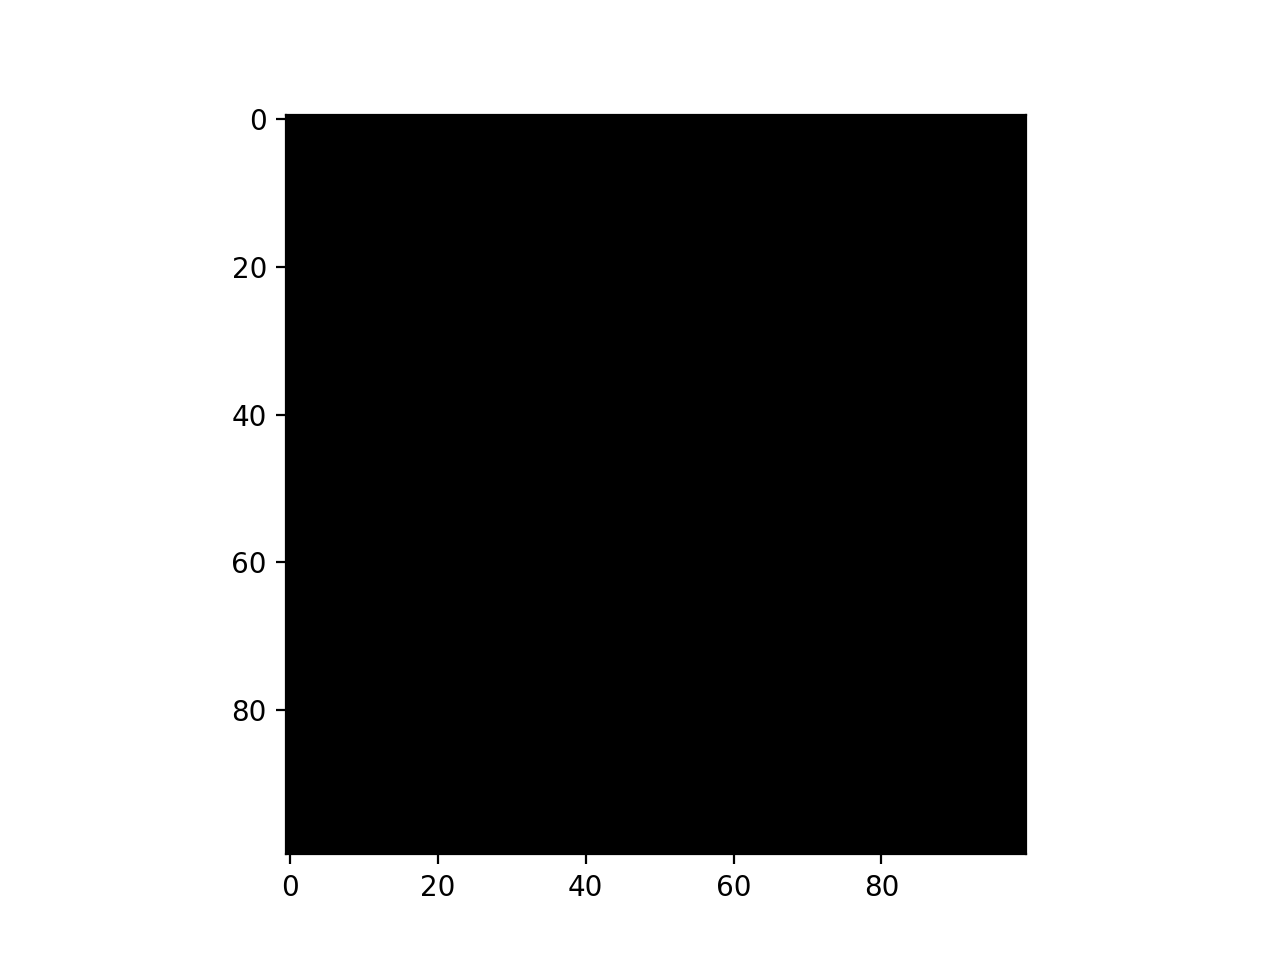
\includegraphics[width=65mm]{figures/ising2d_0.png}
}
\subfloat[10 sweeps]{
  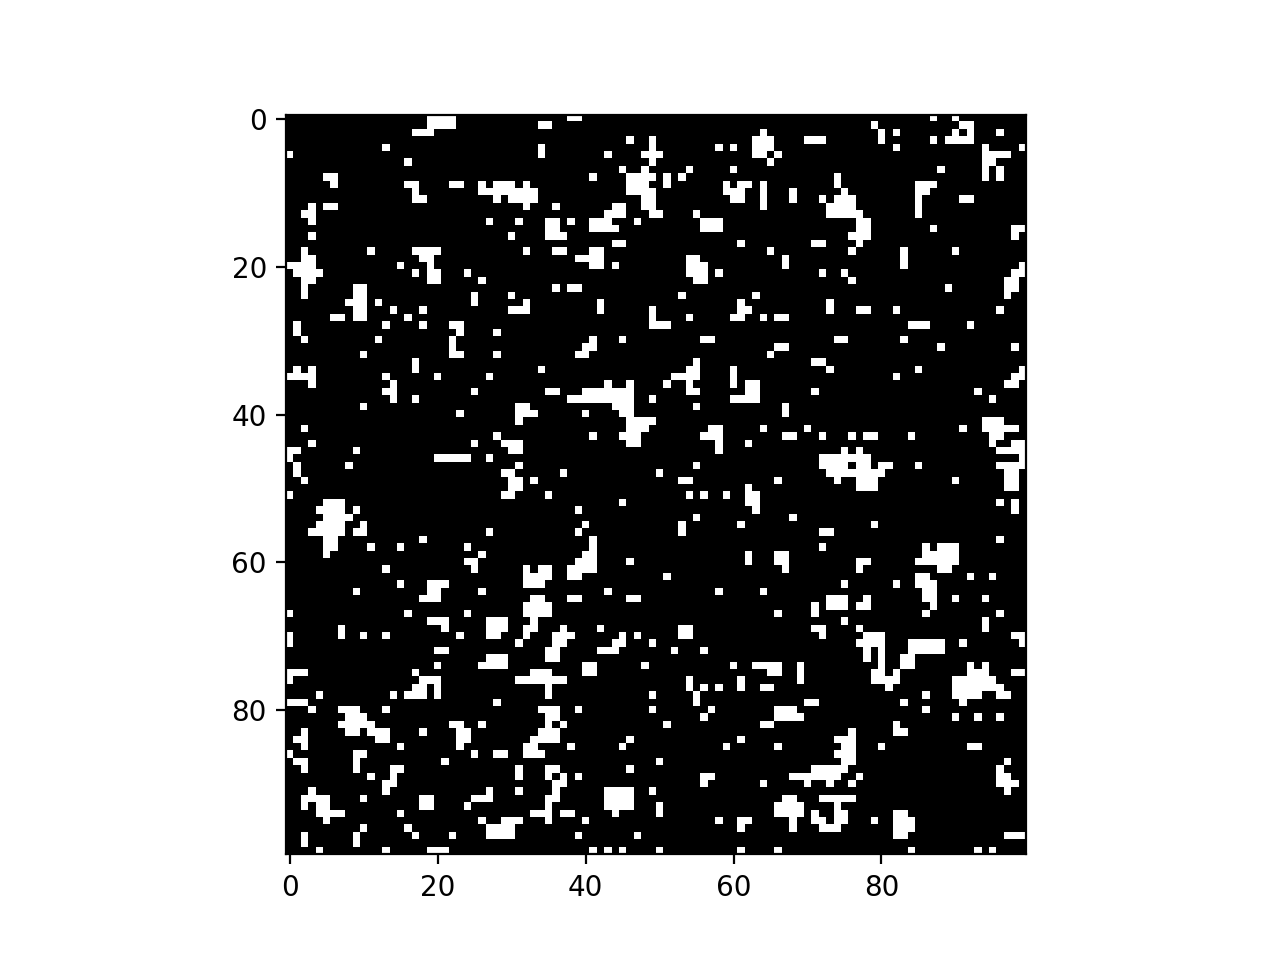
\includegraphics[width=65mm]{figures/ising2d_100000.png}
}
\hspace{0mm}
\subfloat[20 sweeps]{
  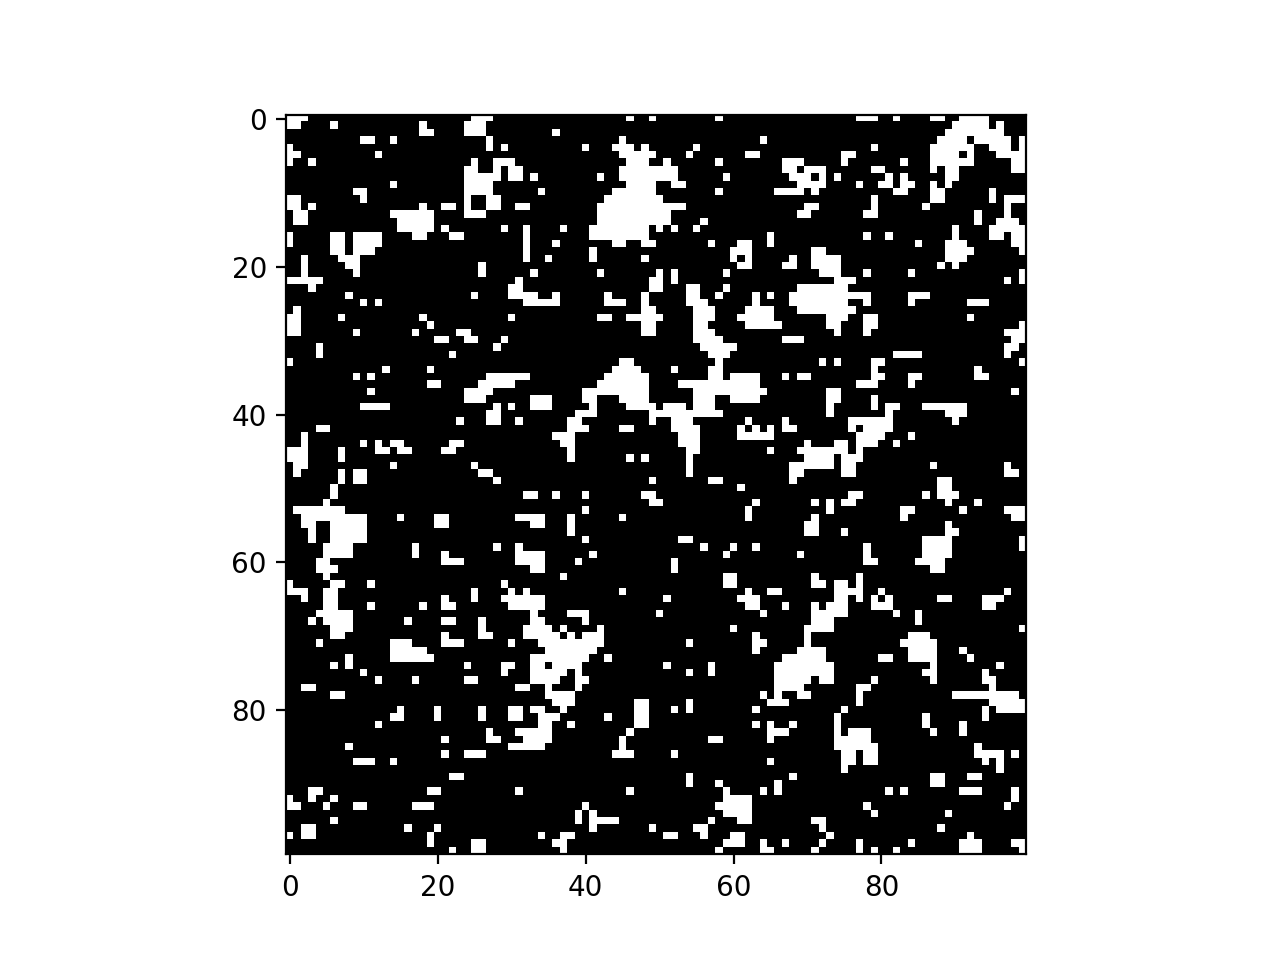
\includegraphics[width=65mm]{figures/ising2d_200000.png}
}
\subfloat[40 sweeps]{
  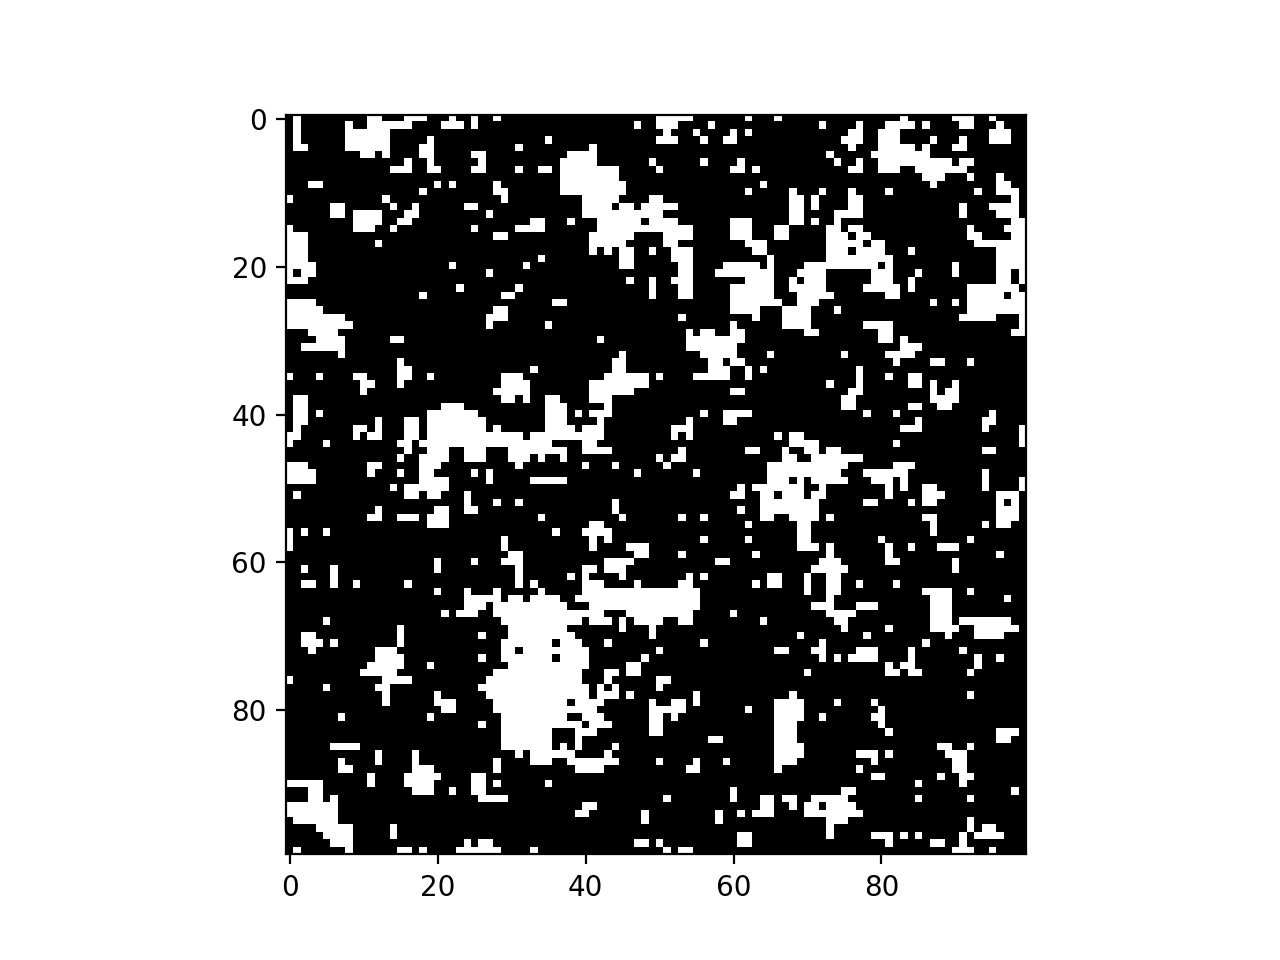
\includegraphics[width=65mm]{figures/ising2d_400000.png}
}
\hspace{0mm}
\subfloat[60 sweeps]{
  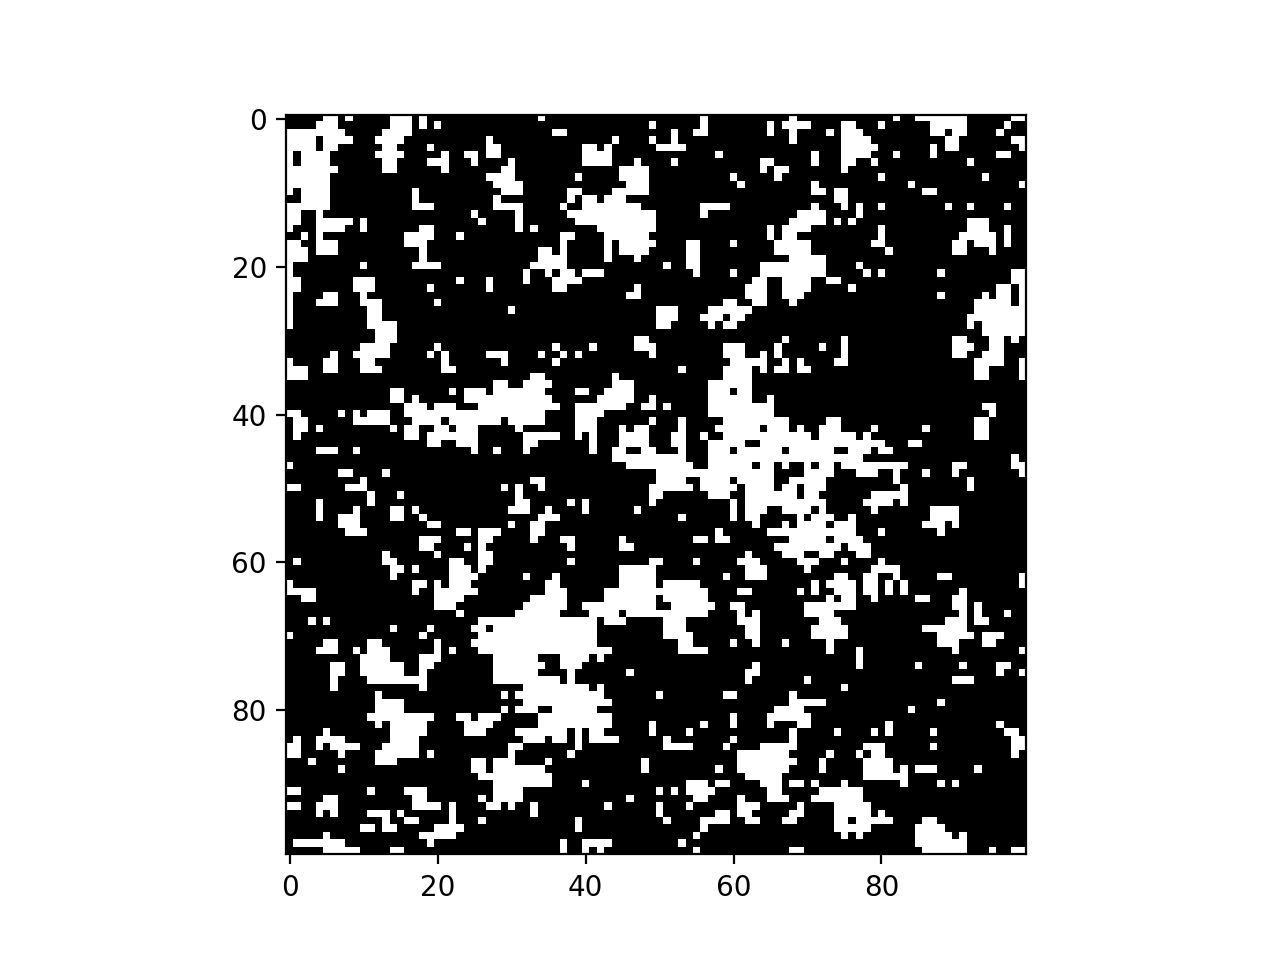
\includegraphics[width=65mm]{figures/ising2d_600000.png}
}
\subfloat[100 sweeps]{
  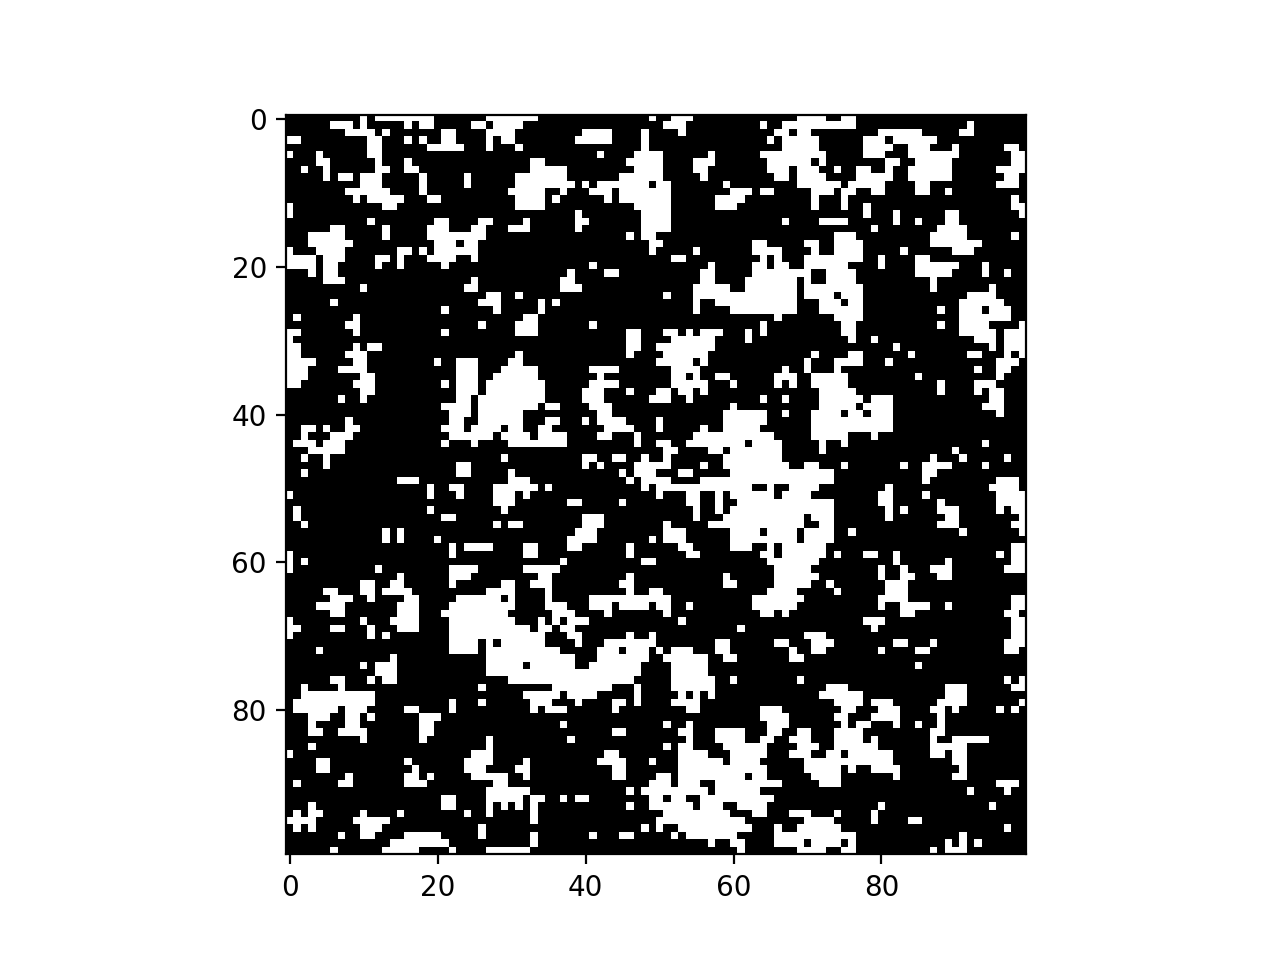
\includegraphics[width=65mm]{figures/ising2d_1000000.png}
}

\end{figure}
\begin{figure} \ContinuedFloat
%\hspace{0mm}
\subfloat[200 sweeps]{
  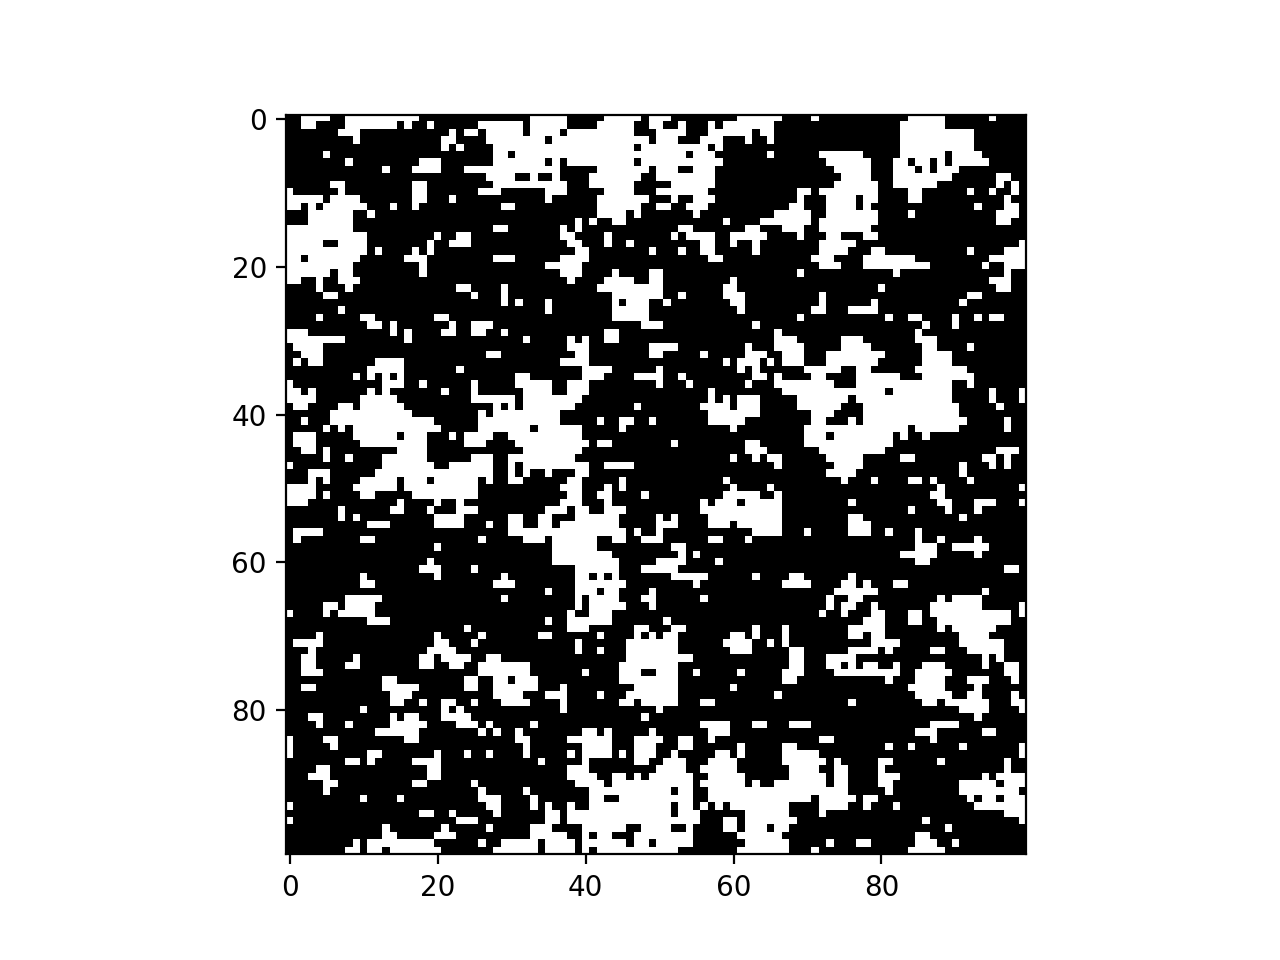
\includegraphics[width=65mm]{figures/ising2d_2000000.png}
}
\subfloat[400 sweeps]{
  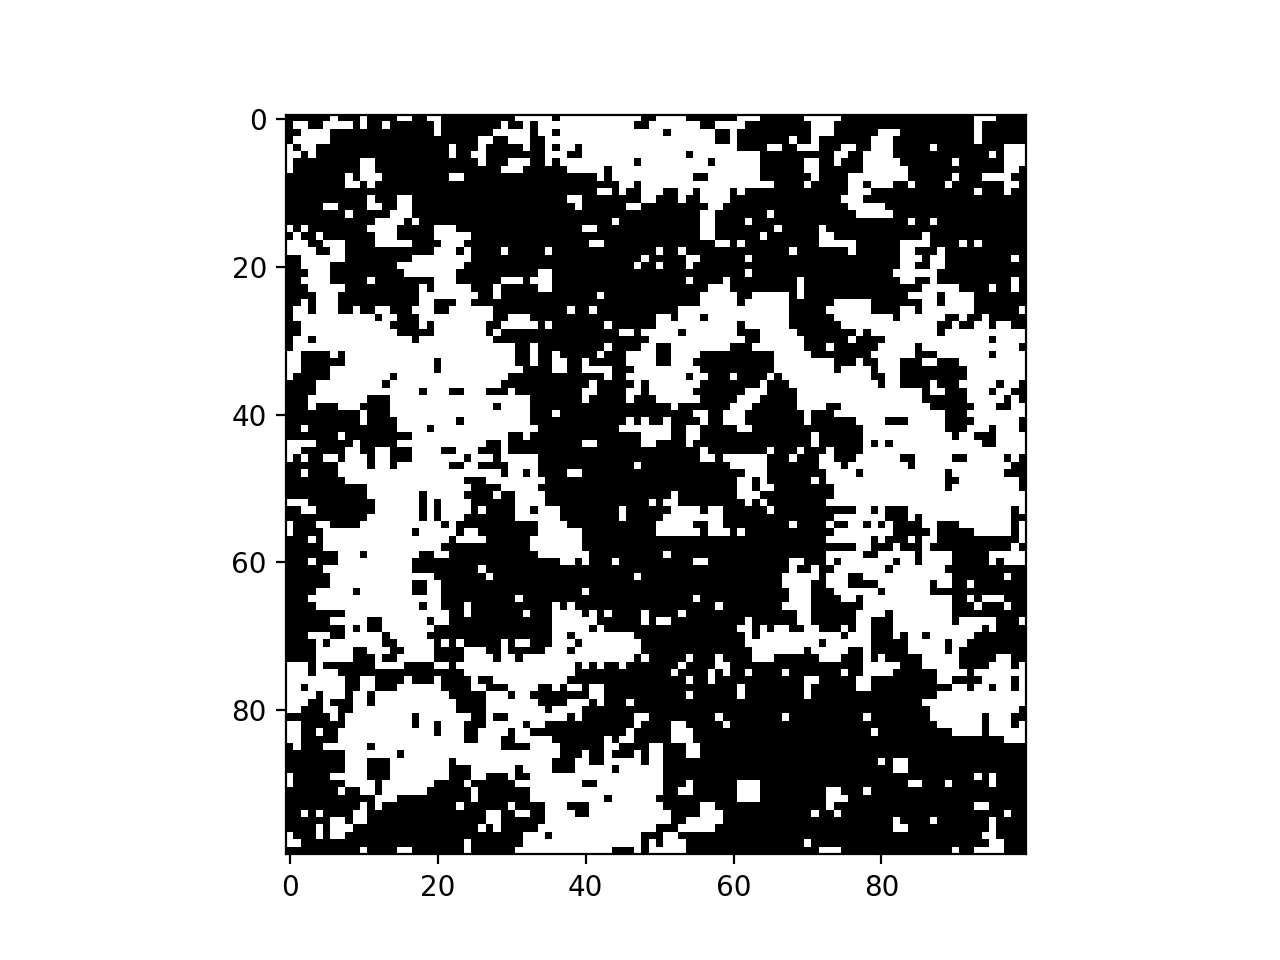
\includegraphics[width=65mm]{figures/ising2d_4000000.png}
}
\hspace{0mm}
\subfloat[1000 sweeps]{
  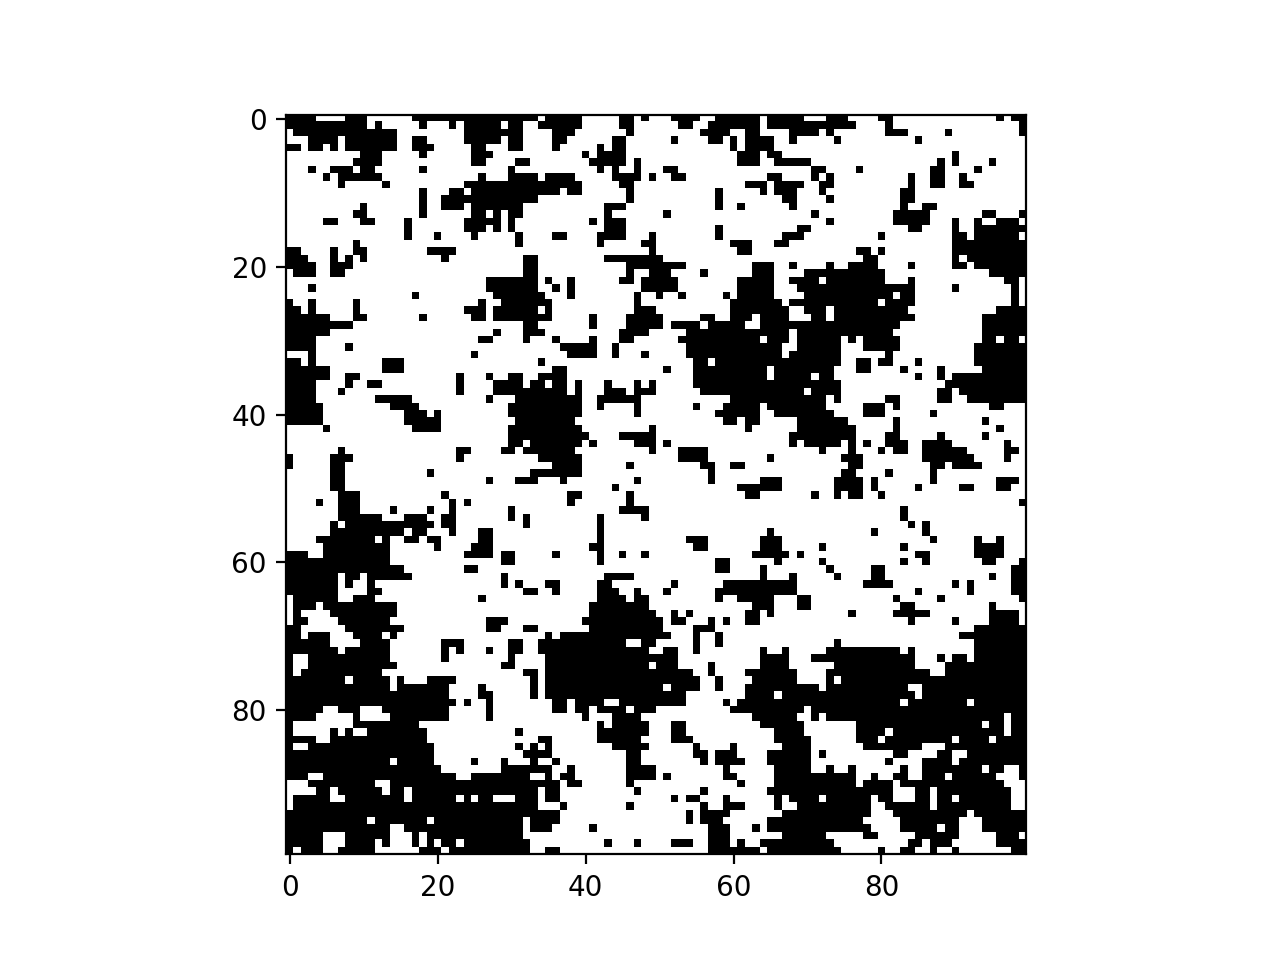
\includegraphics[width=65mm]{figures/ising2d_10000000.png}
}
\caption{$100 \times 100$ 2D Ising model with $J=1$ coming to equilibrium from
initial temperature $T = 0$ to final temperature $T = 2.4$. Spin up is represented
by black squares. }
\end{figure}

\begin{figure}
%\hspace{0mm}
\subfloat[Trial 1]{
  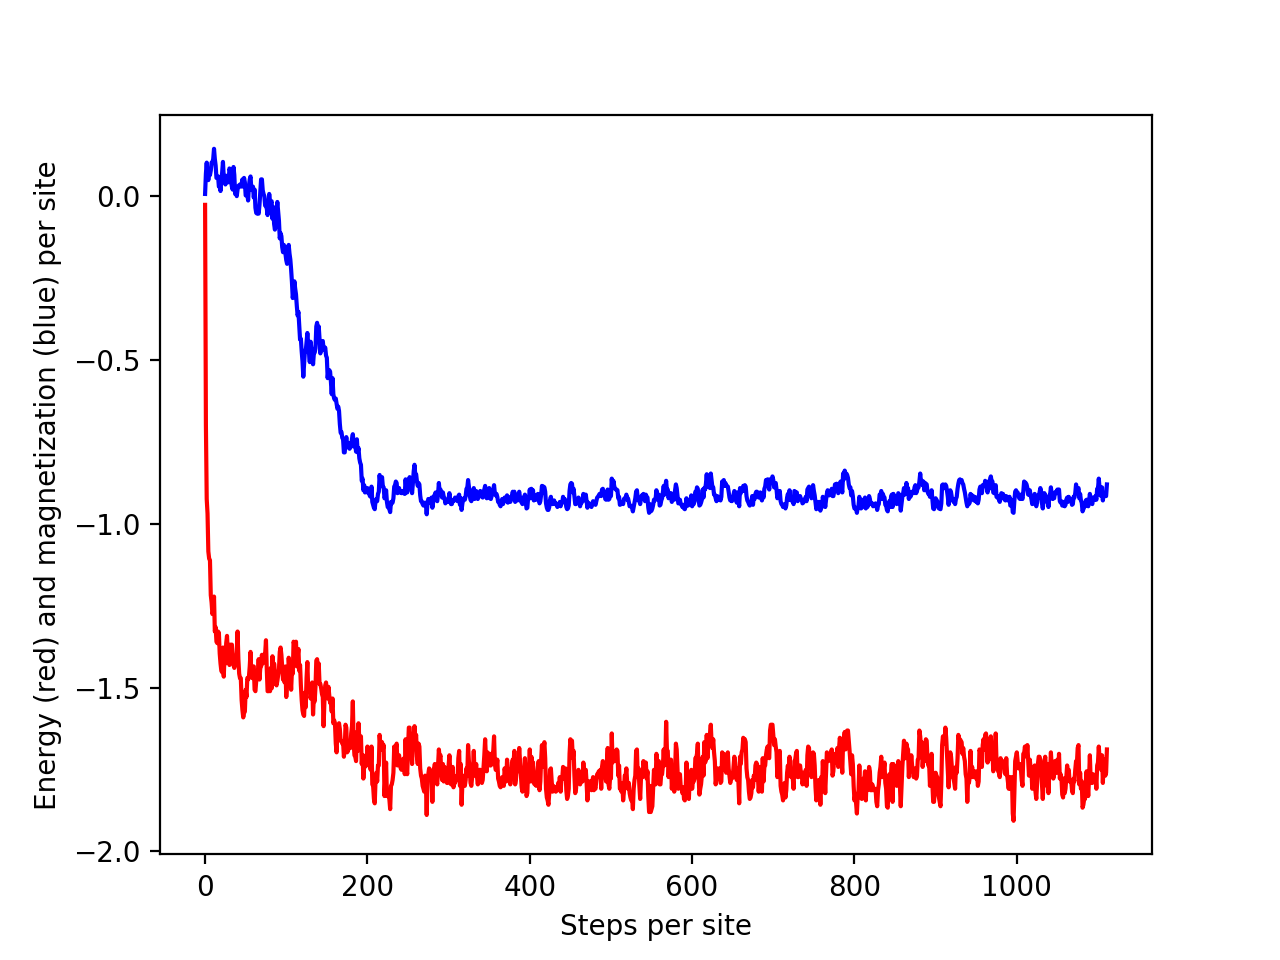
\includegraphics[width=65mm]{figures/mag_energy_1_3030.png}
}
\subfloat[Trial 2]{
  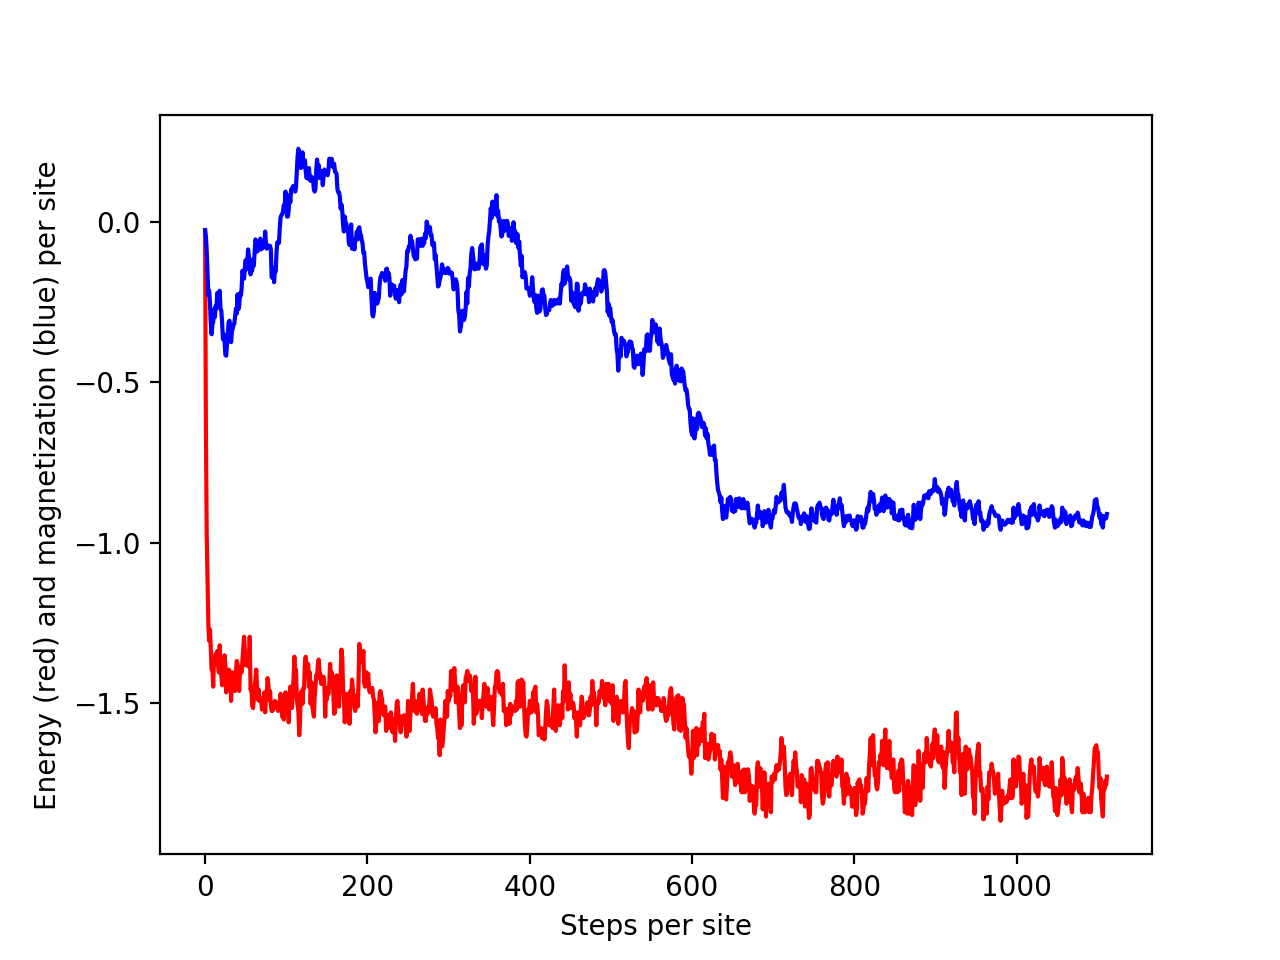
\includegraphics[width=65mm]{figures/mag_energy_2_3030.png}
}
\hspace{0mm}
\subfloat[Trial 3]{
  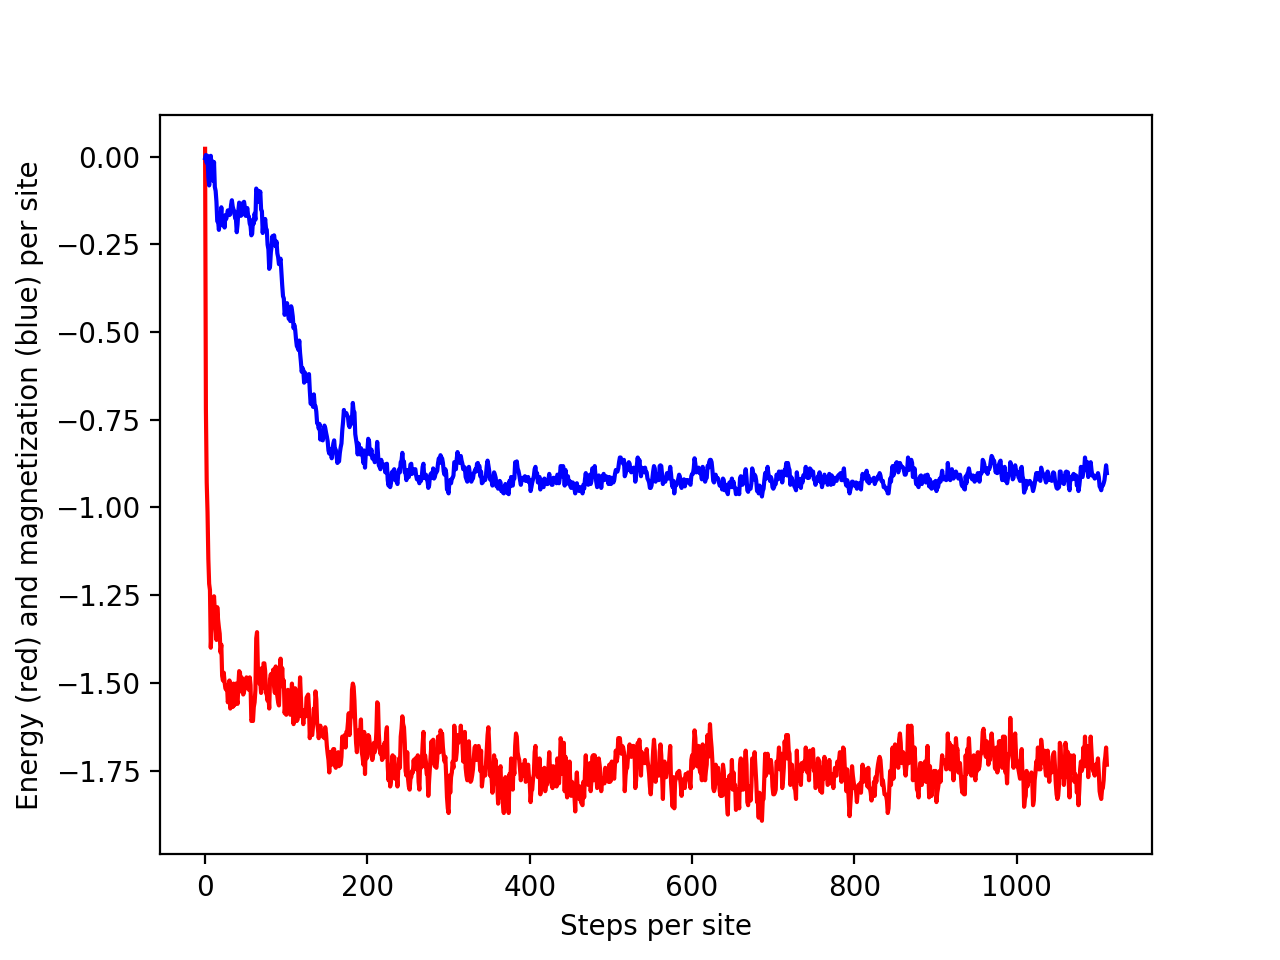
\includegraphics[width=65mm]{figures/mag_energy_3_3030.png}
}
\subfloat[Trial 4]{
  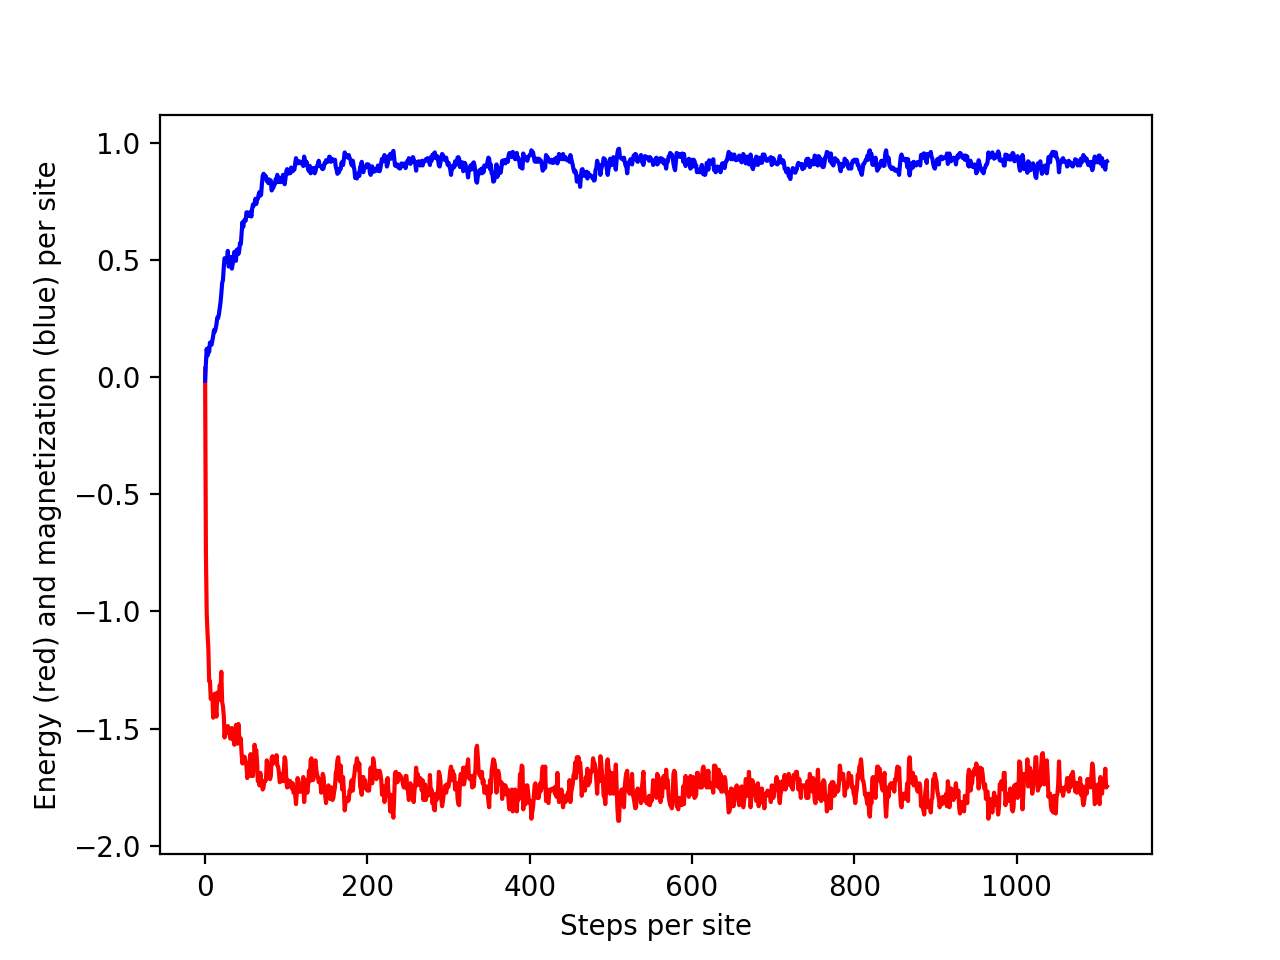
\includegraphics[width=65mm]{figures/mag_energy_4_3030.png}
}
\caption{Magnetization (blue) and internal energy (red) per site of $30 \times 30$
2D Ising model with J=1. Simulation is initialized with random configuration
($T = \infty$) and cooled to $T=2.0$. Four separate trials are presented here.}
\end{figure}

\begin{figure}
%\hspace{0mm}
\subfloat[Trial 1]{
  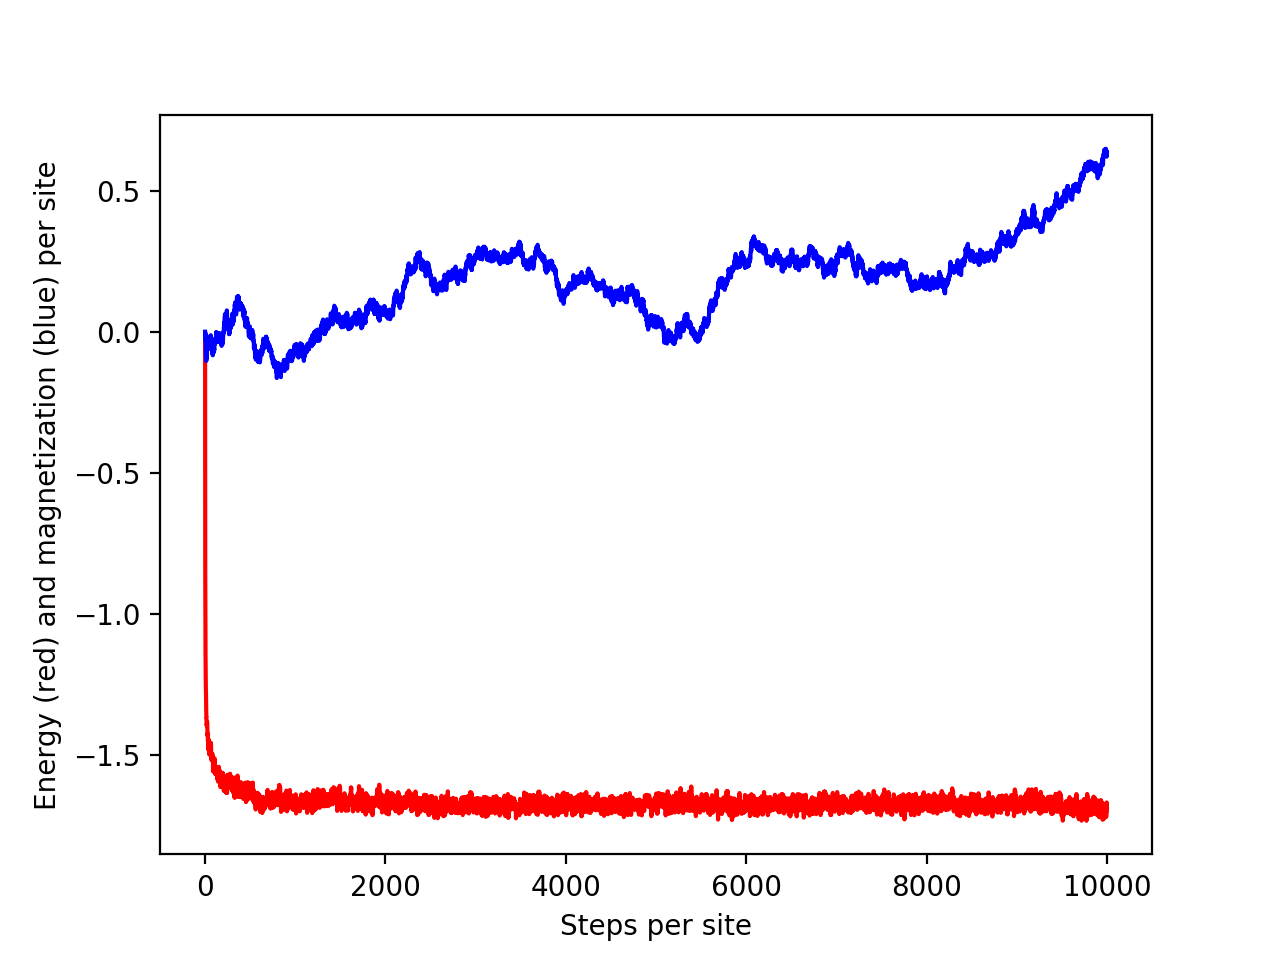
\includegraphics[width=65mm]{figures/mag_energy_1_100100.png}
}
\subfloat[Trial 2]{
  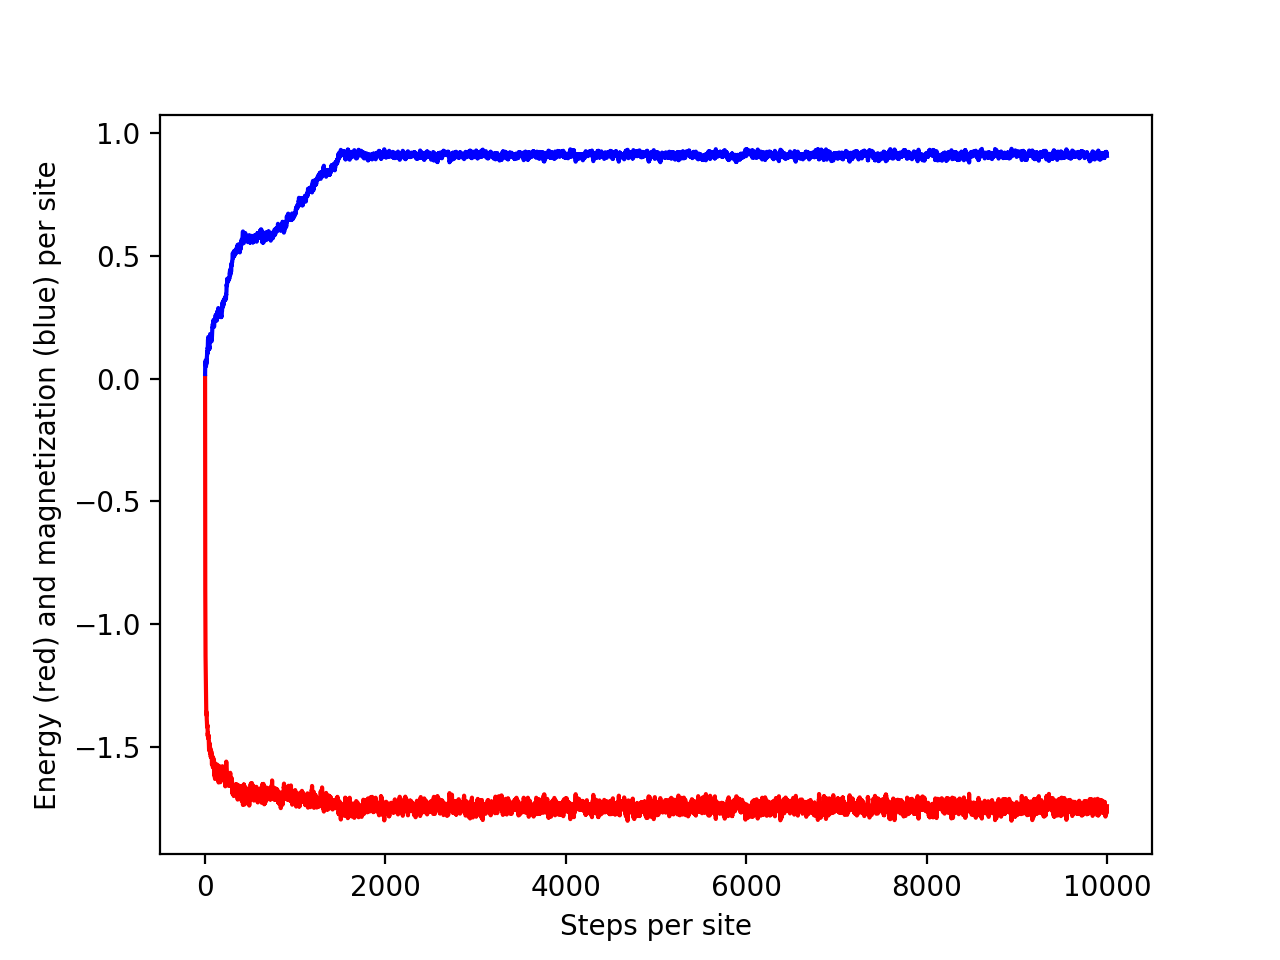
\includegraphics[width=65mm]{figures/mag_energy_2_100100.png}
}
\hspace{0mm}
\subfloat[Trial 3]{
  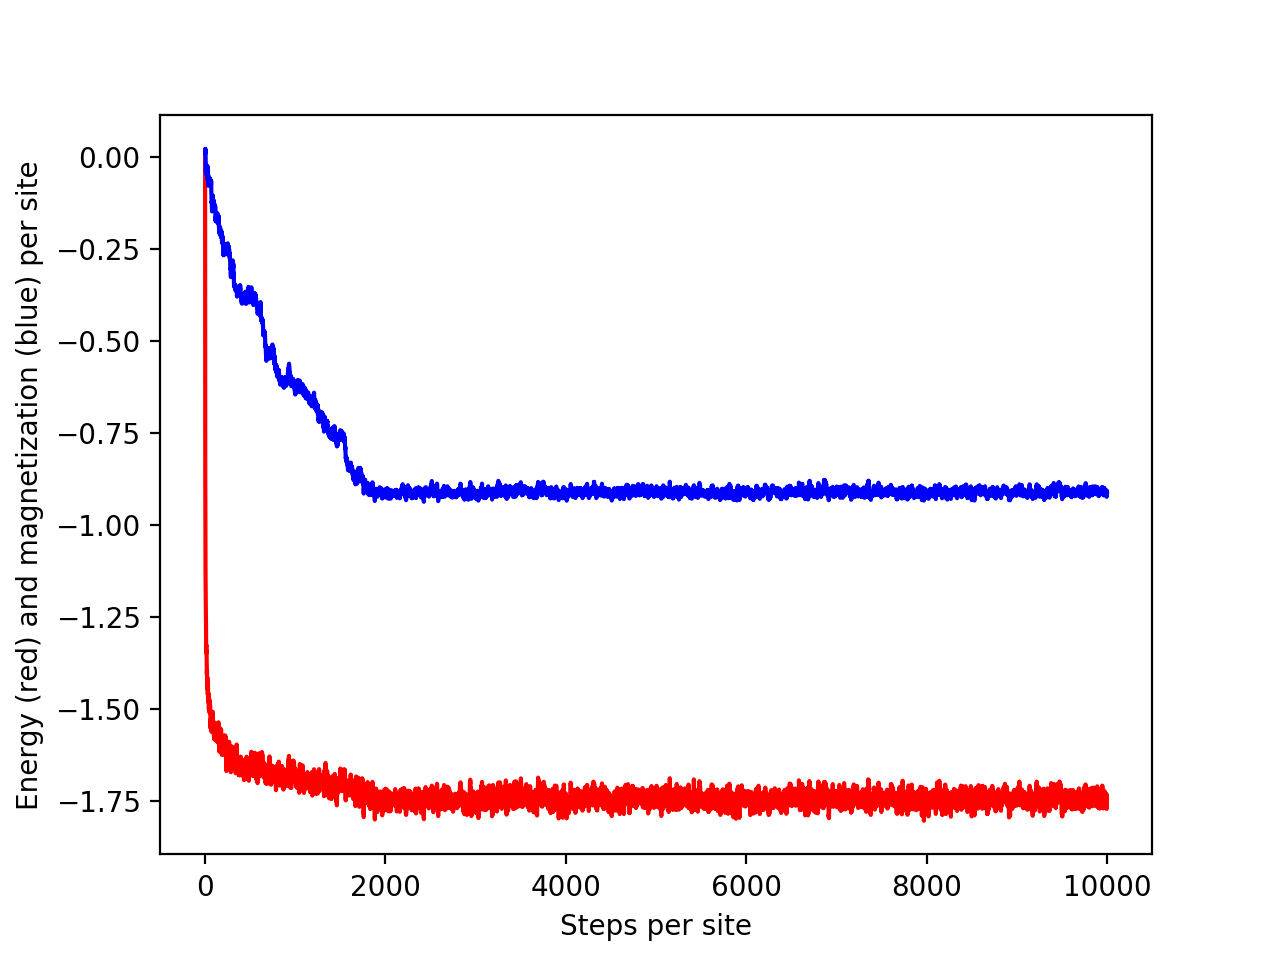
\includegraphics[width=65mm]{figures/mag_energy_3_100100.png}
}
\subfloat[Trial 4]{
  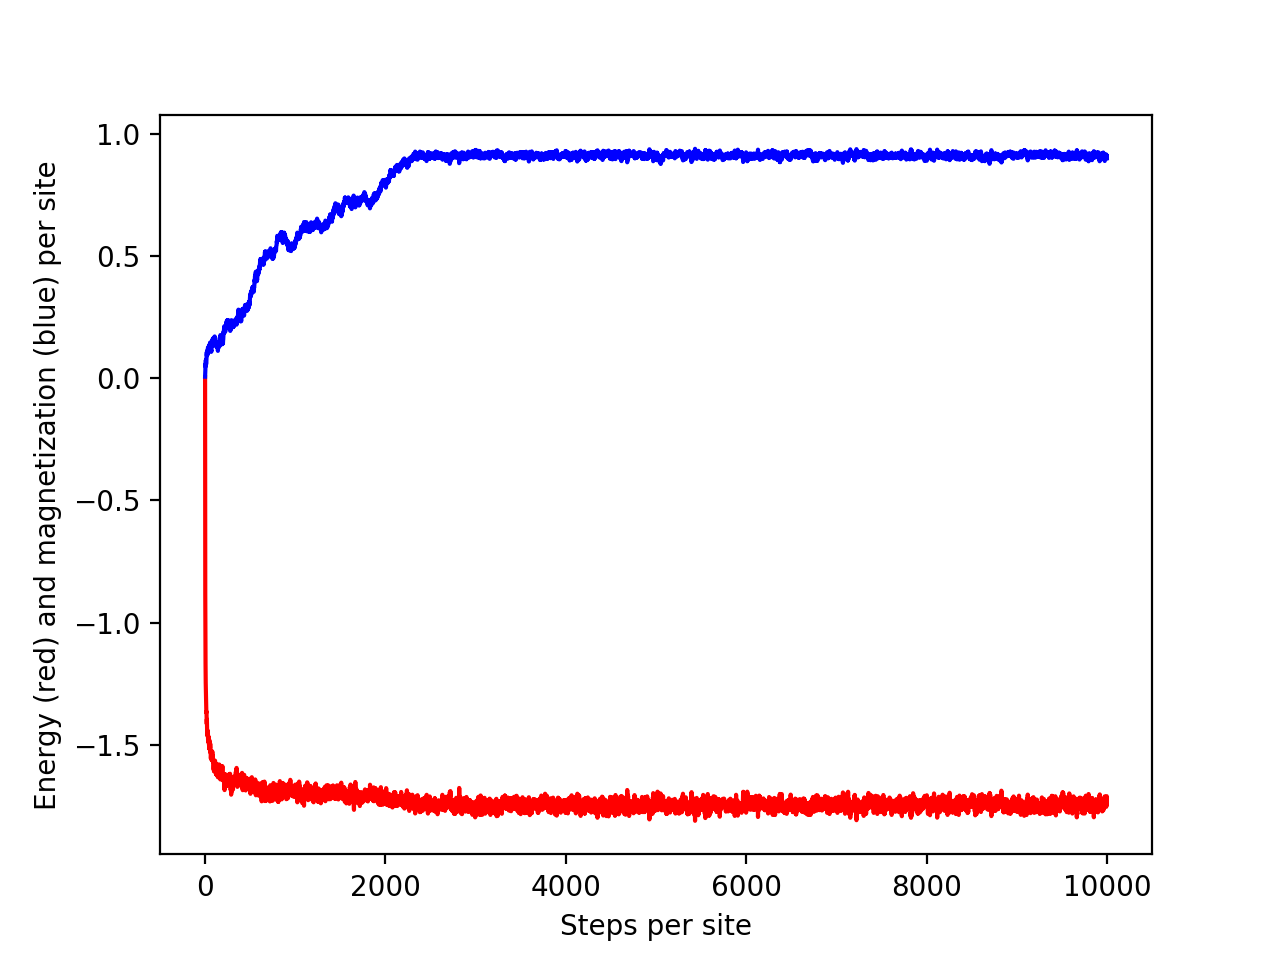
\includegraphics[width=65mm]{figures/mag_energy_4_100100.png}
}
\caption{Magnetization (blue) and internal energy (red) per site of $100 \times 100$
2D Ising model with $J=1$. Simulation is initialized with random configuration
($T = \infty$) and cooled to $T=2.0$. Four separate trials are presented here.}
\end{figure}

% the scale of the autocorrelation has to be much smaller than sample size. Otherwise
% as t increases X(t) is less accurate (fewer samples to integrate over)

\begin{figure}
%\hspace{0mm}
\subfloat[$20 \times 20$ lattice, 25000 sweeps]{
  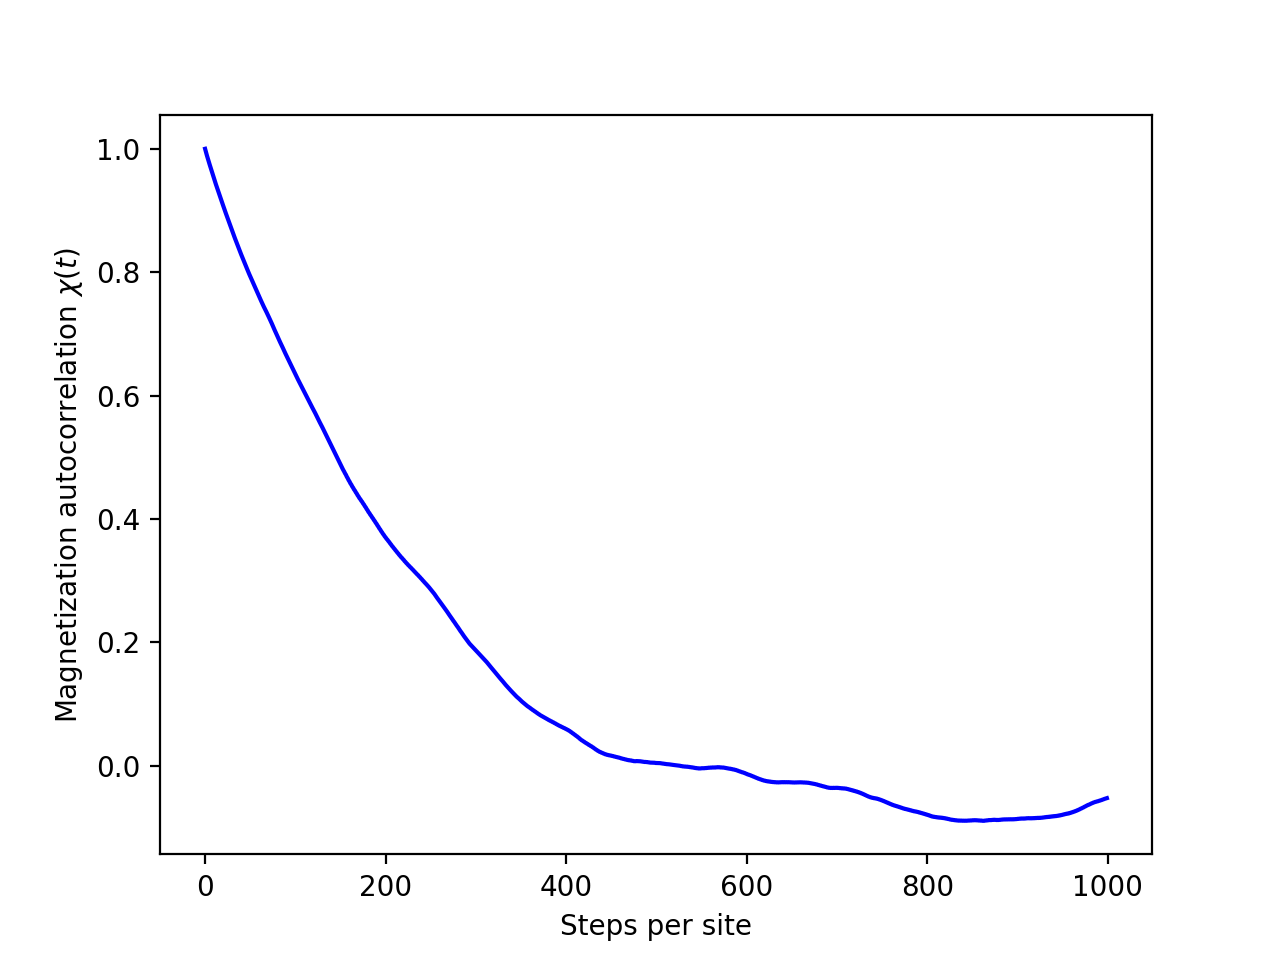
\includegraphics[width=65mm]{figures/autocorrelation_2020_10000000.png}
}
\subfloat[$50 \times 50$ lattice, 40000 sweeps]{
  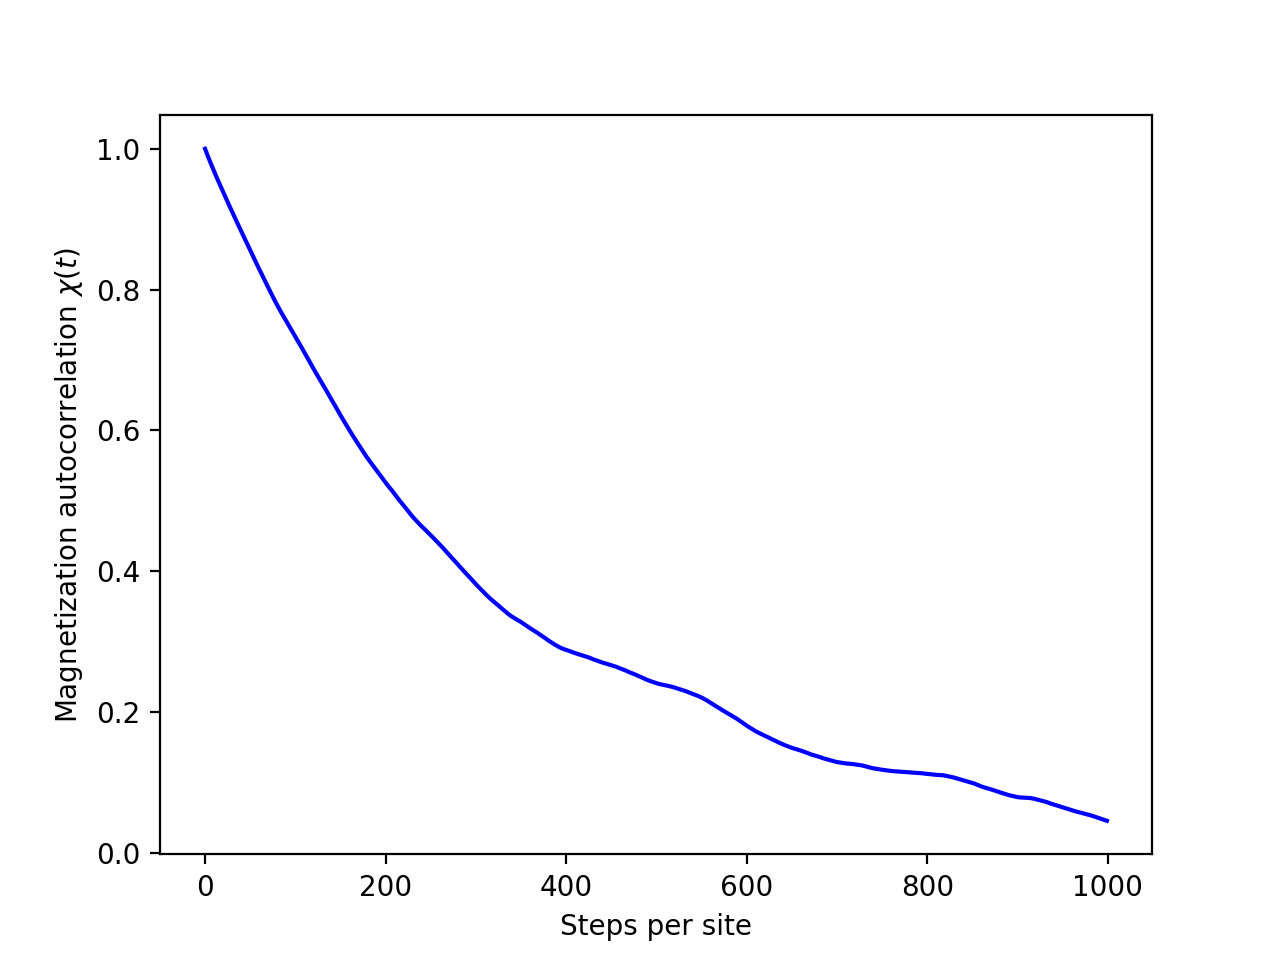
\includegraphics[width=65mm]{figures/autocorrelation_5050_100000000.png}
}

\caption{Magnetization autocorrelation function $\chi(t)$ for 2D Ising Model with
$J=1$. Simulation is initialized with spin-up configuration
($T = 0$) and heated to $T=2.4$.}
\end{figure}




\end{document}
